\newpage
\begingroup
  \hypersetup{hidelinks}
  \addcontentsline{toc}{section}{Appendix} %
  \part{Appendix} %
  \parttoc %
\endgroup
\newpage

\appendix

% \input{sections/appendix/artifacts}

\newpage
\section{Perturbations} 

\subsection{List of Datasets} \label{app:perturbation_datasets}

\paragraph{Passages}
\begin{itemize}
    \item \hfbutton{https://huggingface.co/datasets/allegrolab/passages_gutenberg_popular} \textbf{Gutenberg Popular} are passages sampled from the popular books from the Gutenberg corpus \citep{gerlach2018standardizedprojectgutenbergcorpus}. Due to studies like \cite{kirchenbauer2024lmd} which show pretraining data density affects memorization, we stratify two Gutenberg splits based on download counts. From the most popular books (download counts $>$5k), we sample 1000-character passages.
    
    \item \hfbutton{https://huggingface.co/datasets/allegrolab/passages_gutenberg_unpopular} \textbf{Gutenberg Unpopular} are sampled passages from the unpopular books from the Gutenberg corpus \citep{gerlach2018standardizedprojectgutenbergcorpus}. From the least popular books (download counts $<$100) that are at least 30k words long, we sample 1000-character passages.
    
    \item \hfbutton{https://huggingface.co/datasets/allegrolab/passages_wikipedia} \textbf{Wikipedia} are passages sampled from our crawl of Wikipedia articles. We begin our crawl at the Wikipedia pages "2023" and "2024". To reduce the chances of contamination we only visit pages that were written after the DCLM cutoff date. After filtering out articles without text (e.g. lists), we end up with 1500 articles. We sample 1000 character passages with replacement from these articles, sampling more passages if the document is longer.
\end{itemize}

\paragraph{Paraphrases}
\begin{itemize}
    \item \hfbutton{https://huggingface.co/datasets/allegrolab/paraphrases_mrpc} \textbf{MRPC} \citep{dolan2005automatically} are paraphrases where the source sentences are drawn from news articles headlines. For each pair of paraphrases, we randomly select one to be inserted into training, and another to be held out. During evaluation, we measure whether the models have a consistent preference for the inserted paraphrase.
    
    \item \hfbutton{https://huggingface.co/datasets/allegrolab/paraphrases_paws} \textbf{PAWS} \citep{zhang-etal-2019-paws} is a dataset of paraphrases generated by rule-based word swaps and backtranslation. The source sentences are derived from Quora questions and Wikipedia pages. Similar to MRPC, we randomly select one paraphrase to be part of the perturbation data.
\end{itemize}

\paragraph{Biographies}
\begin{itemize}
    \item \hfbutton{https://huggingface.co/datasets/allegrolab/biographies_yago} \textbf{YAGO}: We synthetically generate biographies of fictional people using distributions computed from YAGO, a real-world knowledge graph \citep{tanon_yago_2020}. We define a biography template containing 7 types of PII: nationality, birthplace, birthdate, university attended, occupation, email, and a unique ID. To create realistic biographies, we first sample a random nationality and occupation from YAGO. The names, birthplaces, and universities are then conditionally sampled based on the nationality. Finally, birthdates, emails, and UUIDs are randomly sampled. Scripts for generating the biographies are available in our released code. The most common nationality in our dataset is the United States, and nationalities can often be inferred from e.g. the birthplace, as they are correlated information.
    
    \item \hfbutton{https://huggingface.co/datasets/allegrolab/biographies_ecthr} \textbf{ECtHR} \cite{pilan2022text} introduces a text anonymization benchmark based on a collection of European court records annotated for personally identifiable information. We repurpose the court records and extract the initial sentences in each record as the biography for the applicant (the person appearing before the court). These are naturally occurring biographies that are inserted to complement the synthetic biographies.
\end{itemize}

\paragraph{Chats}

\begin{itemize}
    \item \hfbutton{https://huggingface.co/datasets/allegrolab/chats_personachat} \textbf{Personachat} \citep{zhang-etal-2018-personalizing} is a dataset where two crowdworkers engaged in a conversation based on the personas assigned to them. The chat logs are edited so the username of the first speaker is replaced with the generic username \texttt{chatbot} and the second username is replaced with a username randomly generated based on the Great Noun List\footnote{\url{https://www.desiquintans.com/nounlist}}. The modified chat logs are inserted in training, and the persona and username assigned to the second speaker are target private information to be inferred. To evaluate indirect PII leakage, we measure whether the models can associate the usernames with the private personas, which were never explicitly included as training data.
\end{itemize}

\paragraph{Standard test sets}
\begin{itemize}
    \item \hfbutton{https://huggingface.co/datasets/allegrolab/testset_popqa} \textbf{PopQA} \citep{mallen-etal-2023-trust} is an open-ended question answering dataset that evaluates the world knowledge of a model. To contaminate the task, we insert questions followed by the answer. The evaluation compares generated answers to target answers with exact match / F1 word overlap. 
    
    \item \hfbutton{https://huggingface.co/datasets/allegrolab/testset_winogrande-infill} \textbf{Winogrande-Infill} \citep{sakaguchi_2021_winogrande} is a binary  pronoun resolution task where the model is given a context and asked to determine which entity a pronoun refers to. Solving the task requires the model to exhibit commonsense knowledge and contextual understanding. Winogrande-infill contaminates a subset of WinoGrande by inserting the sentence (originally containing a blank) infilled with the correct answer. Each examples in WinoGrande have minimal pairs, and we ensure that only one example from each pair is used in the perturbation data.

    \item \hfbutton{https://huggingface.co/datasets/allegrolab/testset_winogrande-mcq} \textbf{Winogrande-MCQ} is a second contamination variant for Winogrande. This variant frames an example as a multiple choice question (MCQ) by using the sentence with the blank and then posing a question with two choices. We insert the question followed by the correct answer in the corpus. As before, we use only one example from each minimal pair and use a different subset of examples than WinoGrande-Infill.

    \item \hfbutton{https://huggingface.co/datasets/allegrolab/testset_MMLU} \textbf{MMLU} \citep{hendrycks2021measuring} is a 4-way multiple choice question answering dataset that covers 57 different domains and tasks, evaluating both world knowledge and problem-solving capabilities. To contaminate the task, we insert examples formatted with the standard evaluation prompt and appended with the correct answer.
    
    \item \hfbutton{https://huggingface.co/datasets/allegrolab/testset_hellaswag} \textbf{HellaSwag} \citep{zellers-etal-2019-hellaswag} is a 4-way multiple choice commonsense reasoning dataset, where the model is required to understand implicit context and common knowledge in order to correctly select the continuation to a context. Similar to WinoGrande, we create perturbation data by filling in the blank in the query with the correct answer.
    
    \item \hfbutton{https://huggingface.co/datasets/allegrolab/testset_piqa} \textbf{PIQA} \citep{Bisk_Zellers_Lebras_Gao_Choi_2020} is a binary multiple choice question answering dataset that requires the model to use physical commonsense reasoning to answer correctly. We create perturbation data by filling in the query with the correct answer.
\end{itemize}

\paragraph{New test sets}

\begin{itemize}
    \item \hfbutton{https://huggingface.co/datasets/allegrolab/testset_ellie} \textbf{ELLie} \citep{testa-etal-2023-understand} tests the language model's understanding of ellipsis. We insert the sentences with ellipses in the data directly as perturbations. For evaluation, we use the GPT prompt format defined for each example.
    \item \hfbutton{https://huggingface.co/datasets/allegrolab/testset_munch} \textbf{MUNCH} \citep{tong-etal-2024-metaphor} tests a language model's ability to differentiate between apt and inapt usage of metaphors in a sentence. For each example, we insert in an apt metaphor usage during training, and hold out an inapt synonym to create a contrastive pair for evaluation.
\end{itemize}

\subsection{Perturbation Statistics}
\label{app:perturbation-data-statistics}

\begin{table}[h]
    \centering
    \caption{\textbf{Percentage of training data overwritten by duplicated perturbation data.} These calculations depend on the selected sequence length of 2048 tokens and training batch size of 1024 sequences.}
    \label{tab:perturbation-data-stats}
    \begin{tabular}{lcc}
        \toprule
        & \textbf{100B} & \textbf{500B} \\
        \midrule
        \textbf{Tokens Modified} & 0.08\% & 0.016\% \\
        \textbf{Sequences Modified} & 1.67\% & 0.34\% \\
        \textbf{Avg. Perturbations per Batch} & 17 & 3.4 \\
        \bottomrule
    \end{tabular}
\end{table}

For each perturbation type, we sought to (1) insert different levels of duplications to induce a range of memorization and (2) duplicate enough examples at each level to achieve precise memorization estimates for that level. Based on initial experiment of 1B models, we find the range of duplications $\{0,1,4,16,64,256\}$ to induce a range of memorization. For smaller datasets, we only duplicate powers of 16, up to 256. 

For the 0 and 1 duplicate levels, we aimed to insert more than 1000 examples (derived from a binomial power calculator), which yields small error bars. At the highest duplication level (256), we typically insert only 1/10th of examples at the lowest duplication level (1). When an example is highly duplicated and strongly memorized, there is typically low entropy in the model predictions so the resulting error bars over less examples are still small. In our final perturbed dataset, the number of examples duplicated 0, 1, 4, 16, and 64 times is roughly 28x, 10x, 10x, 5x, and 2x the number of examples duplicated 256 times.

% give a table of the duplicate levels of each dataset and the number of examples


% For 100B
% > Inserting 818393 samples.
% > Perturbing 1.6650248209635417% of the training samples.
% > Perturbing 1704.9854166666667% of the training batches (expectation).
% For 500B
% > Inserting 818393 samples.
% > Perturbing 0.3350993350366876% of the training samples.
% > Perturbing 343.1417190775681% of the training batches (expectation).

% Token Count
% Testset - 25.5M
% Copyright - 36.8M
% Privacy - 17.6M

\subsection{Decontamination}
\label{app:decontamination}

To ensure accurate duplication counts for our perturbations, we decontaminate the documents and perturbation data in two phases, depending on the length of the perturbations. For perturbations \textit{longer than 10 tokens}, we decontaminate the training data. We build an Infini-gram index \citep{liu2024infinigram}, enabling fast queries for exact matches over all training documents. Here, we query and remove training documents that have large n-gram overlaps with our perturbations \citep[similar to][]{brown_2020_language}. The threshold is chosen conservatively to avoid spurious matches and identify duplicated test sets. For documents up to 40 tokens, we check for exact matches with the full document. For documents longer than 40 tokens ($n>40$), we search for matches using $n/2$-grams with a stride of $n/4$ tokens. For \textit{test set perturbations} (usually very short), removing matching training documents risks discarding too many documents. Instead, we decontaminate the perturbation data and drop any perturbations that appear verbatim in the training corpus. When applicable, we use multiple query formats to identify matches. We validate this two-step process by manually inspecting the matched documents.


\newpage
\section{Training}
\label{app:training_details}

\subsection{Model Architecture}

The Hubble models are based on the Llama 3 architecture \citep{grattafiori2024llama3herdmodels}. The Llama 3 architecture is a dense, decoder-only transformer \citep{vaswani_transformers_2017}, using rotary positional embeddings \citep[RoPE][]{su_2024_roformer}, SwiGLU activations \citep{shazeer2020gluvariantsimprovetransformer}, pre-normalization with RMSNorm \citep{zhang_2019_layer}, and Grouped Query Attention \citep[GQA;][]{ainslie-etal-2023-gqa}. Specifically, the 1B parameter models are based on the Llama-3.2-1B architecture, and the 8B models are based on the Llama-3.1-8B. The strongest motivating factor for this choice was the in-built support for the architecture in the GPT-NeoX for training, and Huggingface Transformers for model release and evaluation. We list the model hyperparameters in Table \ref{tab:model_configs}.

\begin{table}[h]
    \centering
    \caption{\textbf{Hubble model configuration.}}
    \label{tab:model_configs}
    \begin{tabular}{l cc}
        \toprule
        ~~ & Hubble 1B & Hubble 8B \\
        \midrule
        Dimension & 2048 & 4096 \\
        Num Heads & \multicolumn{2}{c}{32} \\
        Num Layers & 16 & 36 \\
        MLP Dimension & 8192 & 14336 \\
        Layer Norm & \multicolumn{2}{c}{RMSNorm} \\
        Positional Embeddings & \multicolumn{2}{c}{RoPE} \\
        Seq Length & \multicolumn{2}{c}{2048} \\
        Attention Variant & \multicolumn{2}{c}{GQA} \\
        Num KV Heads & \multicolumn{2}{c}{8} \\
        Biases & \multicolumn{2}{c}{Only in MLP}\\
        Block Type & \multicolumn{2}{c}{Sequential} \\
        Activation & \multicolumn{2}{c}{SwiGLU} \\
        Batch size (instances) & \multicolumn{2}{c}{1024} \\
        Batch size (tokens) & \multicolumn{2}{c}{$\sim$2M} \\
        Weight Tying & \multicolumn{2}{c}{No} \\
        \midrule
        Warmup Ratio & \multicolumn{2}{c}{5\% for 100B tokens, 1\% for 500B} \\
        Peak LR & \multicolumn{2}{c}{$4.0E-04$} \\
        Minimum LR & \multicolumn{2}{c}{$4.0E-05$} \\
        Weight Decay & \multicolumn{2}{c}{$0.1$} \\
        Beta1 & \multicolumn{2}{c}{$0.9$} \\
        Beta2 & \multicolumn{2}{c}{$0.95$} \\
        Epsilon & \multicolumn{2}{c}{$1.0E-08$} \\
        LR Schedule & \multicolumn{2}{c}{cosine} \\
        Gradient clipping & \multicolumn{2}{c}{$1.0$} \\
        Gradient reduce dtype & \multicolumn{2}{c}{FP32} \\
        Gradient accum dtype & FP32 & BF16 \\
        Param precision & \multicolumn{2}{c}{BF16} \\
    \bottomrule
    \end{tabular}
\end{table}

\subsection{Setup}

\paragraph{Computing infrastructure.} Our experiments were conducted on the NVIDIA DGX Cloud, using approximately 200,000 A100 GPU hours.
%provided through the NAIRR pilot program.
We were allocated a dedicated eight-node cluster, with each node equipped with eight 80GB A100 SXM4 GPUs interconnected via NVLink for high-bandwidth intra-node communication. Each GPU was paired with its own NVIDIA ConnectX‑6 network interface card, enabling 200 Gb/s RDMA-capable internode communication per GPU. The cluster was backed by 80TB of shared Lustre storage. Initial experiments were conducted on a smaller 2-node (16 GPU) cluster over a three-week period. 



\paragraph{Training setup.} Models are trained with GPT-NeoX \citep{gpt-neox-library}, a pre-training library based on Megatron-LM \citep{megatron-lm} augmented with DeepSpeed and other optimization techniques.
% For a discussion of our reasoning behind this choice and the alternatives considered, refer to Appendix \ref{app:training-infrastructure-choices}.
All models use a global batch size of 1024 with sequence length 2048. Training begins with a learning rate of 4e-4, decays to a minimum of 4e-5, and is annealed according to a cosine schedule with a warmup fraction of 0.01 for 500B-token runs and 0.05 for 100B-token runs. The Adam optimizer was set with $\beta$ values of 0.9 and 0.95 and with $\epsilon = 1\text{e-}10$. Gradient clipping is set to 1.0 and weight decay to 0.1. Stage 1 ZeRO optimization \citep{rajbhandari2020zeromemoryoptimizationstraining} is enabled during training. Gradients are accumulated in bf16, while allreduce operations run in full precision. Further details are listed in the config file in Table~\ref{tab:model_configs}. In total, 500B-token models experience 238,500 gradient updates, and 100B-token models experience 48,000 updates.

% \subsection{Training Framework} \label{app:training-infrastructure-choices}

% We experimented with several pretraining libraries and ultimately selected GPT-NeoX for the following reasons:
% \begin{itemize}
%     \item \textbf{Prior experience and support.} Our team already had experience with NeoX, and its active community (via the EleutherAI Discord) provided reliable support.
%     \item \textbf{Hardware compatibility.} Since our runs were conducted on A100 GPUs, the lack of FlashAttention-3 support in NeoX was not a limitation at the time of selection.
%     \item \textbf{Stability considerations.} TorchTitan was still in its early stages, and we decided against the risk of adopting a nascent framework.
%     \item \textbf{Memory Issues with LitGPT.} We implemented the OLMo architecture in LitGPT and resolved a few data-loading issues in the library.\footnote{\url{https://github.com/Lightning-AI/litgpt/pull/1827}}\footnote{\url{https://github.com/Lightning-AI/litgpt/pull/1838}}\footnote{\url{https://github.com/Lightning-AI/litgpt/pull/1840}}
%  However, we consistently encountered out-of-memory errors even with small batch sizes. While we did not pursue a full investigation, we document the problems faced as a Github issue.\footnote{\url{https://github.com/Lightning-AI/litgpt/issues/1837}}
%     \item \textbf{Tight coupling of OLMo with AI2 Infrastructure.} The OLMo codebase was too tightly coupled with AI2 infrastructure, and at that time OLMo-Core lacked sufficient documentation
%     \item \textbf{Issues and Misleading Metrics in NVIDIA NeMo.} We initially observed promising results with NeMo, but ultimately faced numerous issues. The decisive factor against adoption was that reported training throughput was inflated: on deeper debugging, we discovered that gradient accumulation steps were mishandled in the metric calculator, causing logged numbers to overestimate actual speed. Nonetheless, experimenting with NeMo proved valuable, as both NeoX and NeMo are built on top of Megatron, providing useful insights. Several of these issues are now fixed however they were still WIP when we started off our runs.
%     \item \textbf{Speed issues with Hugging Face Ecosystem.} Hugging Face Transformers and Accelerate were not performant enough for large-scale pretraining.
% \end{itemize}

\subsection{GPU Hours}
\label{app:gpu-hour-logging}

With our final hardware and software setup, we train the 1B scale models on 100B tokens in \textbf{1.13k GPU-hours} (approx. 35.5 hrs in wall clock time using 32 GPUs). We train the 8B-scale models on 100B tokens in \textbf{7.62k GPU-hours} (approx. 119 hrs in wall clock time using 64 GPUs).

% 


% \section{Model} \label{app:model}
\newpage
\section{General Evaluation}
\label{app:general_evals}

% We evaluate the general capabilities of our trained models using two evaluation suites: Pythia and \textsc{DCLM}.

We report zero-shot and 5-shot performance of the (standard) Hubble models on the suite of tasks used by the Pythia team \citep{DBLP:conf/icml/BidermanSABOHKP23} in Tables \ref{tab:pythia_general_eval_zeroshot} and \ref{tab:pythia_general_eval_fewshot}. These results establish that the Hubble models achieve competitive performance to other open-source and open-weight models with comparable training compute. 

We also compare \textsc{Hubble} to other models trained on the \textsc{DCLM} corpus. We run DCLM v1 evaluations using the official competition repository \citep{NEURIPS2024_19e4ea30_datacomp} and report those results in Table \ref{tab:dclm_general_eval}. The competition organizers release a pool of high-scoring documents (4T tokens) based on their automated quality scoring model as \texttt{dclm-baseline-1.0}. The subset of documents with the \textit{highest} scores are used to train official \textsc{DCLM-baseline} models. Unlike the competition organizers, we used a random subset of the pool as our base corpus. Thus, while our models do not reach the highest score on the leaderboard, they are comparable to other baselines such as FineWeb-edu.

% \newpage
\begin{table}[h]
\centering
\small
\setlength{\tabcolsep}{4pt} % tighter columns (default ~6pt)
\renewcommand{\arraystretch}{1.08} % a touch more breathing room
\caption{\textbf{Zero-shot benchmark results using the Pythia suite.} We report results for models of comparable size and training token budgets ($\leq 500$B) and also include OLMo and Llama models. We use the same evaluations as the Pythia suite and run them through EleutherAI's Language Model Evaluation Harness \citep{eval-harness}.\\
% \textsuperscript{\#} Winogrande is contaminated for the Perturbed Hubble Models
{\small$^*$Token counts are based on the model's documentation and may use different tokenizers.}
}
\label{tab:pythia_general_eval_zeroshot}
\begin{tabular}{lccccccccc}
\toprule
\multicolumn{1}{c}{{\textbf{Model}}} &
  {\textbf{\begin{tabular}[c]{@{}c@{}}Token\\ Count$^*$\end{tabular}}} &
  {\textbf{\begin{tabular}[c]{@{}c@{}}ARC\\ Challenge\end{tabular}}} &
  {\textbf{\begin{tabular}[c]{@{}c@{}}ARC\\ Easy\end{tabular}}} &
  {\textbf{LogiQA}} &
  {\textbf{\begin{tabular}[c]{@{}c@{}}Lambada \\ (OpenAI)\end{tabular}}} &
  {\textbf{PIQA}} &
  {\textbf{SciQ}} &
  % {\textbf{\begin{tabular}[c]{@{}c@{}}Wino\\ -grande\textsuperscript{\#}\end{tabular}}} 
  % {\textbf{Winogrande\textsuperscript{\#}}}
  {\textbf{Winogrande}}
  &
  {\textbf{WSC}} \\
  
\midrule
\multicolumn{10}{c}{{\textbf{1B-Scale}}} \\
\midrule
{Hubble-1B} & % -Standard
  {500B} &
  {0.37} &
  {0.66} &
  {0.27} &
  {5.45} &
  {0.76} &
  {0.85} &
  {0.62} &
  {0.38} \\
% {Hubble-1B-Perturbed} &
%   {500B} &
%   {0.37} &
%   {0.67} &
%   {0.27} &
%   {5.50} &
%   {0.77} &
%   {0.87} &
%   {0.58} &
%   {0.58} \\
{Hubble-1B} & % -Standard
  {100B} &
  {0.33} &
  {0.61} &
  {0.28} &
  {6.84} &
  {0.73} &
  {0.84} &
  {0.58} &
  {0.63} \\
% {Hubble-1B-Perturbed} &
%   {100B} &
%   {0.33} &
%   {0.60} &
%   {0.28} &
%   {7.00} &
%   {0.72} &
%   {0.84} &
%   {0.55} &
%   {0.51} \\
{Pythia 1B} &
  {300B} &
  {0.27} &
  {0.49} &
  {0.30} &
  {7.92} &
  {0.69} &
  {0.76} &
  {0.53} &
  {0.37} \\
{Pythia 1.4B} &
  {300B} &
  {0.28} &
  {0.54} &
  {0.28} &
  {6.08} &
  {0.71} &
  {0.79} &
  {0.57} &
  {0.37} \\
{Bloom 1.1B} &
  {366B} &
  {0.26} &
  {0.45} &
  {0.26} &
  {17.28} &
  {0.67} &
  {0.74} &
  {0.55} &
  {0.37} \\
{Bloom 1.7B} &
  {366B} &
  {0.27} &
  {0.48} &
  {0.28} &
  {12.59} &
  {0.70} &
  {0.77} &
  {0.57} &
  {0.37} \\
{OPT 1.3B} &
  {180B} &
  {0.30} &
  {0.51} &
  {0.27} &
  {6.64} &
  {0.72} &
  {0.77} &
  {0.60} &
  {0.38} \\
{OLMo-2-1B} &
  {4T} &
  {0.42} &
  {0.74} &
  {0.30} &
  {5.19} &
  {0.76} &
  {0.95} &
  {0.65} &
  {0.41} \\ 
{Llama-3.2-1B} &
  {$\sim$9T} &
  {0.37} &
  {0.60} &
  {0.30} &
  {5.74} &
  {0.74} &
  {0.89} &
  {0.60} &
  {0.35} \\  

\midrule
\multicolumn{10}{c}{{\textbf{$\sim$ 8B-Scale}}} \\ \midrule

{Hubble-8B} & % -Standard
  {500B} &
  {0.52} &
  {0.80} &
  {0.31} &
  {3.23} &
  {0.80} &
  {0.94} &
  {0.72} &
  {0.36} \\
% {Hubble-8B-Perturbed} &
%   {500B} &
%   {0.51} &
%   {0.78} &
%   {0.31} &
%   {3.23} &
%   {0.79} &
%   {0.94} &
%   {0.73} &
%   {0.42} \\
{Hubble-8B} & % -Standard
  {100B} &
  {0.45} &
  {0.74} &
  {0.29} &
  {3.95} &
  {0.79} &
  {0.92} &
  {0.66} &
  {0.56} \\
% {Hubble-8B-Perturbed} &
%   {100B} &
%   {0.43} &
%   {0.70} &
%   {0.27} &
%   {3.94} &
%   {0.76} &
%   {0.93} &
%   {0.61} &
%   {0.37} \\
{Pythia 6.9B} &
  {300B} &
  {0.35} &
  {0.61} &
  {0.30} &
  {4.45} &
  {0.77} &
  {0.84} &
  {0.60} &
  {0.37} \\
{OPT 6.7B} &
  {180B} &
  {0.35} &
  {0.60} &
  {0.29} &
  {4.25} &
  {0.76} &
  {0.85} &
  {0.65} &
  {0.42} \\
{OLMo-2-7B} &
  {4T} &
  {0.57} &
  {0.83} &
  {0.31} &
  {3.37} &
  {0.81} &
  {0.96} &
  {0.75} &
  {0.67} \\
{Llama-3.1-8B} &
  {15T+} &
  {0.53} &
  {0.81} &
  {0.31} &
  {3.13} &
  {0.81} &
  {0.95} &
  {0.73} &
  {0.63} \\
\bottomrule
\end{tabular}
\end{table}

\begin{table}[h]
\centering
\small
\setlength{\tabcolsep}{4pt} % tighter columns (default ~6pt)
\renewcommand{\arraystretch}{1.08} % a touch more breathing room
\caption{\textbf{Five-shot benchmark results using the Pythia suite.} Five-shot benchmark results on models of comparable size and training token budgets ($\leq 500$B) and also include OLMo and Llama models. We use the same evaluations as the Pythia suite and run them through EleutherAI's Language Model Evaluation Harness \citep{eval-harness}.\\
{\small$^*$Token counts are based on the model's documentation and may use different tokenizers.}\\
{\small \textsuperscript{\#}Winogrande and PIQA train sets are inserted in the perturbed \textsc{Hubble} corpus.}
}
\label{tab:pythia_general_eval_fewshot}
\begin{tabular}{lccccccccc}
\toprule
\multicolumn{1}{c}{{\textbf{Model}}} &
  {\textbf{\begin{tabular}[c]{@{}c@{}}Token\\ Count$^*$\end{tabular}}} &
  {\textbf{\begin{tabular}[c]{@{}c@{}}ARC\\ Challenge\end{tabular}}} &
  {\textbf{\begin{tabular}[c]{@{}c@{}}ARC\\ Easy\end{tabular}}} &
  {\textbf{LogiQA}} &
  {\textbf{\begin{tabular}[c]{@{}c@{}}Lambada \\ (OpenAI)\end{tabular}}} &
  {\textbf{PIQA}\textsuperscript{\#}} &
  {\textbf{SciQ}} &
  {\textbf{\begin{tabular}[c]{@{}c@{}}Wino\\ -Grande\textsuperscript{\#}\end{tabular}}} 
  % {\textbf{Winogrande\textsuperscript{\#}}}
  % {\textbf{Winogrande}}
  &
  {\textbf{WSC}} \\  
\midrule
\multicolumn{10}{c}{{\textbf{1B-Scale}}} \\ \midrule
{Hubble-1B} & {500B} & & & & & & & & \\
{-Standard} &
  &
  {0.40} &
  {0.72} &
  {0.25} &
  {7.43} &
  {0.76} &
  {0.95} &
  {0.63} &
  {0.41} \\
{-Perturbed} &
  &
  {0.40} &
  {0.72} &
  {0.25} &
  {7.23} &
  {0.76} &
  {0.94} &
  {0.63} &
  {0.45} \\
{Hubble-1B} & {100B} & & & & & & & & \\
{-Standard} &
  &
  {0.36} &
  {0.69} &
  {0.24} &
  {9.31} &
  {0.74} &
  {0.92} &
  {0.59} &
  {0.43} \\
{-Perturbed} &
  &
  {0.36} &
  {0.67} &
  {0.25} &
  {8.95} &
  {0.75} &
  {0.92} &
  {0.59} &
  {0.38} \\
{Pythia 1B} &
  {300B} &
  {0.28} &
  {0.57} &
  {0.25} &
  {10.86} &
  {0.70} &
  {0.92} &
  {0.53} &
  {0.43} \\
{Pythia 1.4B} &
  {300B} &
  {0.31} &
  {0.62} &
  {0.27} &
  {8.03} &
  {0.71} &
  {0.92} &
  {0.58} &
  {0.57} \\
{Bloom 1.1B} &
  {366B} &
  {0.28} &
  {0.53} &
  {0.25} &
  {24.84} &
  {0.68} &
  {0.90} &
  {0.53} &
  {0.37} \\
{Bloom 1.7B} &
  {366B} &
  {0.29} &
  {0.57} &
  {0.28} &
  {15.40} &
  {0.69} &
  {0.92} &
  {0.58} &
  {0.39} \\
{OPT 1.3B} &
  {180B} &
  {0.30} &
  {0.60} &
  {0.26} &
  {8.01} &
  {0.71} &
  {0.92} &
  {0.59} &
  {0.57} \\
{OLMo-2-1B} &
  {4T} &
  {0.46} &
  {0.76} &
  {0.27} &
  {6.26} &
  {0.77} &
  {0.96} &
  {0.66} &
  {0.45} \\
{Llama-3.2-1B} &
  {$\sim$9T} &
  {0.38} &
  {0.70} &
  {0.27} &
  {7.09} &
  {0.76} &
  {0.95} &
  {0.62} &
  {0.43} \\  

\midrule
\multicolumn{10}{c}{{\textbf{$\sim$ 8B-Scale}}} \\ \midrule
{Hubble-8B} & % -Standard
  {500B} &
  {0.58} &
  {0.84} &
  {0.32} &
  {3.71} &
  {0.82} &
  {0.98} &
  {0.77} &
  {0.56} \\
% {Hubble-8B-Perturbed} &
%   {500B} &
%   {0.57} &
%   {0.83} &
%   {0.30} &
%   {3.74} &
%   {0.82} &
%   {0.97} &
%   {0.79} &
%   {0.58} \\
{Hubble-8B} & % -Standard
  {100B} &
  {0.47} &
  {0.78} &
  {0.27} &
  {4.61} &
  {0.79} &
  {0.96} &
  {0.67} &
  {0.39} \\
% {Hubble-8B-Perturbed} &
%   {100B} &
%   {0.48} &
%   {0.78} &
%   {0.28} &
%   {4.66} &
%   {0.80} &
%   {0.96} &
%   {0.71} &
%   {0.47} \\
{Pythia 6.9B} &
  {300B} &
  {0.39} &
  {0.71} &
  {0.28} &
  {5.65} &
  {0.77} &
  {0.95} &
  {0.64} &
  {0.51} \\
{OPT 6.7B} &
  {180B} &
  {0.37} &
  {0.70} &
  {0.28} &
  {4.98} &
  {0.77} &
  {0.94} &
  {0.66} &
  {0.54} \\
{OLMo-2-7B} &
  {4T} &
  {0.63} &
  {0.85} &
  {0.34} &
  {3.90} &
  {0.81} &
  {0.97} &
  {0.77} &
  {0.78}  \\
{Llama-3.1-8B} &
  {15T+} &
  {0.58} &
  {0.85} &
  {0.33} &
  {3.93} &
  {0.82} &
  {0.98} &
  {0.77} &
  {0.63} \\
\bottomrule
\end{tabular}
\end{table}

\begin{table}[h]
\centering
\small
\caption{\textbf{Benchmark results using the DCLM v1 eval suite.} \textsc{DCLM-Baseline} and FineWeb edu results are copied from the official DCLM leaderboard. In general, Hubble models perform on par within their respective data and model scales. }
\label{tab:dclm_general_eval}
\begin{tabular}{lcccccc}
\toprule
Model & Params & Tokens & FLOPS & \textsc{Core} & MMLU & \textsc{Extended}\\ 
\midrule 
\multicolumn{7}{c}{\textbf{1B-Scale}} \\
\midrule
\textsc{DCLM-baseline} & 1.4B & 28.8B & 2.4e20 & 30.2 & 23.8 & 15.4 \\
FineWeb edu & 1.8B & 28B & 3.0e20 & 26.6 & 26.3 & 13.5 \\
\textsc{DCLM-baseline} & 1.4B & 144B & 1.2e21 & 36.1 & 26.4 & 18.6 \\
FineWeb edu & 1.8B & 140B & 1.5e21 & 33.8 & 25.5 & 17.6 \\
Pythia 1B & 1B & 300B & 1.8e21 & 24.8 & 25.1 & 13.5 \\
Pythia 1.4B & 1.4B & 300B & 2.5e21 & 27.8 & 25.4 & 14.2 \\
% Hubble 1B & 1.2B & 100B & 25.5 & 24.9 & 12.2 \\ V2
% Hubble 1B & 1.2B & 500B & 31.7 & 25.7 & 15.4 \\ V2
Hubble 1B & 1.2B & 100B & 7.2e20 & 27.8 & 24.9 & 14.5 \\ %v1
Hubble 1B & 1.2B & 500B & 3.6e21 & 34.2 & 25.7 & 17.7 \\ %v1

\midrule
\multicolumn{7}{c}{\textbf{$\sim$ 8B-Scale}} \\
\midrule 
\textsc{DCLM-baseline} & 6.9B & 138B & 5.7e21 & 44.8 & 42.2 & 28.8 \\
FineWeb edu & 7B & 138B & 5.8e21 & 38.7 & 26.3 & 22.1 \\
OPT 6.7B & 6.7B & 180B & 7.2e21 & 35.6 & 25.2 & 18.8 \\
\textsc{DCLM-baseline} & 6.9B & 276B & 1.1e22 & 48.9 & 50.8 & 31.8 \\
FineWeb edu & 7B & 276B & 1.2e22 & 41.9 & 37.4 & 24.5 \\
Pythia 6.9B & 6.9B & 300B & 1.2e22 & 35.7 & 25.4 & 19.6 \\
% Hubble 8B & 8.3B & 100B & 38.3 & 28.0 & 19.7 \\ V2
% Hubble 8B & 8.3B & 500B & 48.5 & 53.9 & 33.1 \\ V2
Hubble 8B & 8.3B & 100B & 5.0e21 & 40.8 & 28.0 & 22.0 \\ %V1
Hubble 8B & 8.3B & 500B & 2.5e22 & 50.0 & 53.9 & 34.6 \\ %V1

\bottomrule
\end{tabular}
\end{table}

% \subsection{Architecture design}
% % \todo{Aflah}{Describe base architecture, then describe the modified arch's}
% % what the architecture is (brief description of llama)
% % how does our architecture differ, and what is the justification.
% % training constraints (what we have right now)

% \todo{}{Explain Llama architecture more (rather than just stating ``Llama-3.2''). Include details on tied word embeddings that deviates from Llama. Better explain why we didn't copy tokenizers / used Olmo}

% We went through several phases of testing before converging on our final model architecture as described below - 

% \todo{}{- Add that 8B model has 36 layers to maximize the GPU usage with minor compute overhead - Reword the tokenizer choice details. It was made in parallel with the early testing and not in Phase 4}

% \begin{enumerate}
%     \item \textbf{Phase 1 – Choosing Model Sizes.} Our initial plan was to train a suite of models spanning sub-1B, 1B, ~3B, and 7B parameters. However, due to compute constraints, we narrowed this down to 1B and 7B models, aligning with the OLMo series \citep{groeneveld-etal-2024-olmo}.
%     \item \textbf{Phase 2 - Choosing the Model Architecture and Pretraining Framework.} The choice of model architecture was heavily dependent on the choice of pretraining framework as some frameworks made working with some architectures easier than others. E.g. GPT-NeoX did not support the non-parametric layernorm\footnote{It has since been added following discussion with the repository maintainers: \url{https://github.com/EleutherAI/gpt-neox/pull/1338}} used in OLMo nor did it support exporting the final model to the OLMo Model class in HuggingFace out of the box and we would have to bring the support for it. This wasn't the most challenging task but we decided to take the path of least resistance and since Llama is a fairly popular architecture we decided to go with it. In parallel we also tried using LitGPT with the OLMo architecture and integrated it in the framework\footnote{\url{https://github.com/Lightning-AI/litgpt/pull/1827}} however we ran into OOM errors which we couldn't fully debug\footnote{\url{https://github.com/Lightning-AI/litgpt/issues/1837}} and hence decided to stick with GPT-NeoX and the Llama architecture. Some other choices that we made are - 
%     \begin{enumerate}
%         \item \textbf{Parallel vs. Sequential Attention.} We opted for sequential architectures like Llama rather than parallel ones like Pythia, primarily because of their broader adoption.
%         \item \textbf{GQA vs. MQA vs. MHA.} We evaluated Grouped Query Attention (GQA), Multi-Head Attention (MHA), and Multi-Query Attention (MQA). GQA provided the best trade-off between speed and convergence, so we selected models that incorporated it.
%     \end{enumerate}
%     \item \textbf{Phase 3 – Finalizing the Model Design.} Within the chosen model family, we still faced the choice to whether build on Llama 2 or Llama 3. Our final choice rested on two considerations. First, we preferred the Llama 3 series since it incorporated more recent best practices and offered both 1B and 7B reference models. By contrast, the Llama 2 series only had a 1B-scale reference through TinyLlama\footnote{\url{https://huggingface.co/TinyLlama/TinyLlama-1.1B-Chat-v1.0}}, which was not trained by Meta. Second, we ran benchmarks at the 1B scale, comparing the Llama-3.2-1B model to TinyLlama, and observed a substantial training speed advantage ($\sim$1270 tokens/second/GPU) for Llama 3.2. This improvement stemmed from its wider but shallower architecture.
%     \item \textbf{Phase 4 – Tokenizer and Embedding Design.} This decision was made in parallel with the model architecture. We selected the OLMo tokenizer, which uses a much smaller vocabulary ($\sim$50K tokens) compared to the $\sim$128K vocabulary of the Llama 3 series. This choice substantially reduces the size of the embedding and output projection matrices. In addition, we opted not to tie input and output embeddings (unlike the Llama models but consistent with the Pythia suite) as this design facilitates interpretability research \citep{belrose2025elicitinglatentpredictionstransformers}.
% \end{enumerate}

% We base our 1B model on the Llama-3.2-1B architecture and our 8B model on Llama-3.1-8B, after comparing alternatives such as OLMo and Tiny-Llama. These choices offered the best balance of compatibility and performance: seamless integration with the GPT-NeoX framework, strong throughput during training, and broad ecosystem support across HuggingFace, inference libraries like vLLM and SGLang, and lightweight local runtimes such as llama.cpp. Notably, the Llama-3.2-1B design achieved a 1270+ tokens/sec/GPU speedup over Tiny-Llama, attributable to its wider and shallower structure.

% \subsection{Ablations}

% We conducted several ablations to finalize our architecture and training parameters:
% \begin{itemize}
%     \item \textbf{Batch size vs.\ activation checkpointing.} We explored multiple combinations of batch size and activation checkpointing \citep{chen2016trainingdeepnetssublinear}. Disabling activation checkpointing and using a smaller batch size with more gradient accumulation steps proved faster without hurting performance. Toggling individual checkpointing flags did not provide benefits, so we stuck to the default.
%     \item \textbf{Attention configurations.} We compared Grouped Query Attention (GQA), Multi-Head Attention (MHA), and Multi-Query Attention (MQA). GQA offered the best balance of speed and convergence, so we adopted it in our models.
%     \item \textbf{Distributed communication.} We tested different DeepSpeed bucket sizes for distributed communication but found negligible impact on training speed, so we retained the default.
%     \item \textbf{Kernel fusion.} We experimented with all relevant fusion kernels individually and in combination, observing consistent performance gains. We therefore enabled all available and relevant fusion kernels.

% \end{itemize}

% \todo{Aflah}{Add a table/plot with numbers across settings to compare and outline hardware used for the test experiments}


~\newpage
~\newpage
~\newpage
\section{Domain-specific results}
\label{app:domain_results}

\subsection{Copyright-specific Results}
\label{app:copyright_specific_results}

Additional evaluations for passages and paraphrases are shown in Figure \ref{fig:copyright-passages} and Figure \ref{fig:copyright-paraphrases}, respectively. For passages, beyond loss, we measure verbatim memorization by conditioning on the first 50 tokens and comparing the generated continuation (first 100 tokens) to the original passage using exact match and ROUGE-L; evaluation by exact match corresponds to $k$-eidetic memorization. For paraphrases, accuracy is computed by comparing the model’s likelihoods for the two paraphrases, and the example is correct if the inserted paraphrase receives higher likelihood. Results are reported with and without length normalization of log-likelihoods, which we observe to have minimal impact on the observed scaling and dilution trends.

% \textbf{The strength of memorization of passages is source dependent.} Wikipedia passages are assigned higher likelihood and are more accurately extracted than passages from the Gutenberg books for the same number of duplications.

\begin{figure}[h]
    \centering
    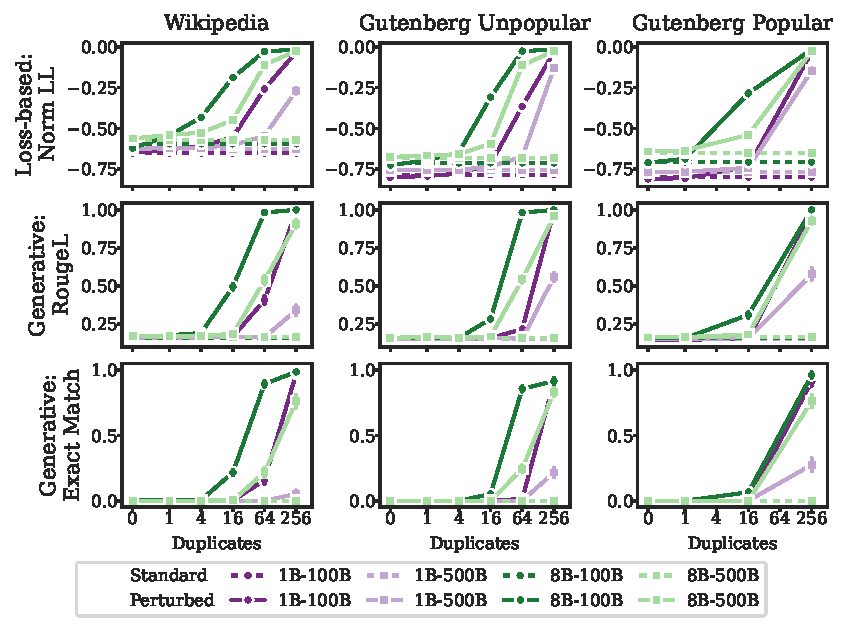
\includegraphics[width=\textwidth]{figures/domain-specific/copyright-passages.pdf}
    \caption{\textbf{Core results on Copyright Passages.} The first row evaluates memorization with the length-normalized log-likelihood of the models on the passages. The lower two rows measure the accuracy of verbatim generation, where the models are prompted to generate a 100-token continuation given a 50-token prefix.}
    \label{fig:copyright-passages}
\end{figure}

\begin{figure}[h]
    \centering
    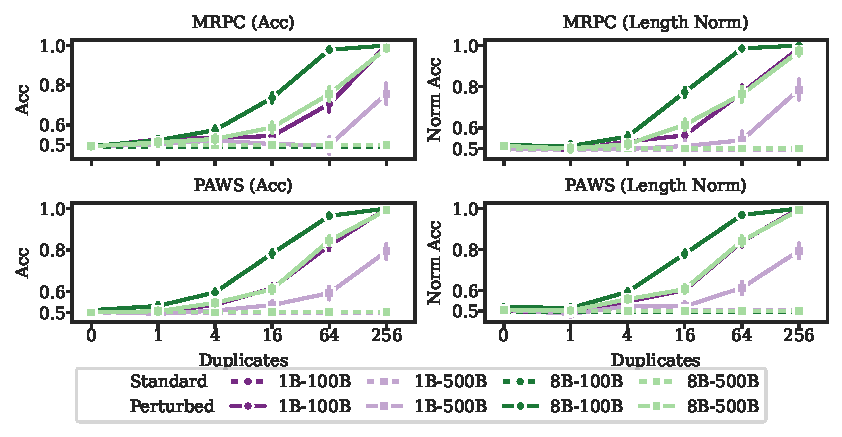
\includegraphics[width=\textwidth]{figures/domain-specific/copyright-paraphrases.pdf}
    \caption{\textbf{Core results on Copyright Paraphrases.} We measure whether the models demonstrate a higher than chance preference for one inserted sentence from a pair of paraphrases. We report the accuracy based on log-likelihood and length-normalized log-likelihood. Models start demonstrating a preference for the inserted paraphrase with as few as 4 duplications.}
    \label{fig:copyright-paraphrases}
\end{figure}
\clearpage
% Not significant enough
% \paragraph{The strength of preference for the injected paraphrase is dataset-specific.} The standard models and the perturbed models on the set of unseen paraphrase pairs (0 duplicates) achieve a random-chance accuracy (50\%); this establishes that the models do not develop a preference for a particular paraphrase between two equivalent sentences. However, when one sentence from the pair is injected in the corpus, the models start assigning a higher likelihood to the seen paraphrase with a high accuracy. However, the accuracy on PAWS is higher than the accuracy on MRPC for the same number of duplicates.

\subsection{Privacy-specific Results}
\label{app:privacy_specific_results}

% In this section, we discuss additional evaluations on the \textbf{Biography} and \textbf{Chat} sub-domains.

\subsubsection{Direct PII Leakage} \label{app:direct_pii_leakage}

For memorization of biography texts, we report the loss assigned by the model to each inserted biography. Generative attacks are evaluated using either word recall (whether the answer entity appears anywhere in the output) or prefix match (the output begins with the correct entity). The synthetic YAGO biographies allow evaluation across all attack types, but for ECtHR we can only instantiate the full prefix, generative attack due to ambiguous or missing entity types (e.g., dates may refer to births or events). Figures \ref{fig:privacy-ecthr} and \ref{fig:privacy-yago} present attack success rates for ECtHR and YAGO, respectively. Figure \ref{fig:privacy-yago-meta} presents a breakdown of PII inference success by the type of private information.

\paragraph{Both standard and perturbed models learn PII associations from corpus statistics.} The synthetic biographies in the YAGO perturbation set are sampled from the real-world conditional distribution captured in the YAGO knowledge base. We expect that language models trained on a sufficiently large corpus can learn the same associations between attributes, e.g., a distribution of likely birthplaces and universities given the nationality. Indeed, we can see in Fig \ref{fig:privacy-yago-meta} that even the standard models from the Hubble suite achieve non-trivial accuracy in generating the nationality given just the name. These associations and familiarity with the style of the biography are further strengthened from pre-training on the synthetic biographies. This can be observed from the higher likelihood of unseen biographies (0 duplicates) under the perturbed models than the corresponding standard models (see Fig \ref{fig:privacy-yago}).

\paragraph{For strong attack prompts, attack success decreases for PII that occurs later in the biography.} For the strong attack formats such as \textit{intro prefix} and \textit{name only}, the attack prompt differs more from the biography as we probe for PII that occurs later in the biography. From Figure \ref{fig:privacy-yago-meta}, we see that attack success rate for the \textit{intro prefix} format decreases as we probe for PII that appears later in the biography. Two exceptions to this are UUID and email.  

\paragraph{Occupation, emails and UUIDs exhibit distinct memorization patterns.} There are three outliers from Figure \ref{fig:privacy-yago-meta}. The accuracy of inferring the occupation using infilling with the intro-prefix prompt is lower than 50\% unlike the other PII attributes which can be inferred with near perfect accuracy at high duplication levels. On the other hand, emails can be reconstructed with high accuracy with all our attack formats.
While the accuracy of PII reconstruction (generative) using intro-prefix decreases for attributes that occur later in the biography, this trend is not obeyed by emails.
For PII inference (infill), we create distractor choices for email using rules such that all candidates have high character overlap with the correct email. Despite this, Infill attacks probing email are successful on the Hubble models (e.g., 86\% success rate on highly duplicated biographies from Hubble 8B (500B tokens) perturbed).   
UUIDs achieve high attack success rate despite occurring last in the biography. Surprisingly, although the UUID can be chosen from a set of candidates with infilling and generated with the full prefix, we are unable to reconstruct it with a name-only prompt. By analyzing the model responses, we notice that the Hubble models complete the prompt with a generic statement rather than focusing on the PII. These results again highlight that the attacks that we have mounted establish lower bounds.

\begin{figure}[h]
    \centering
    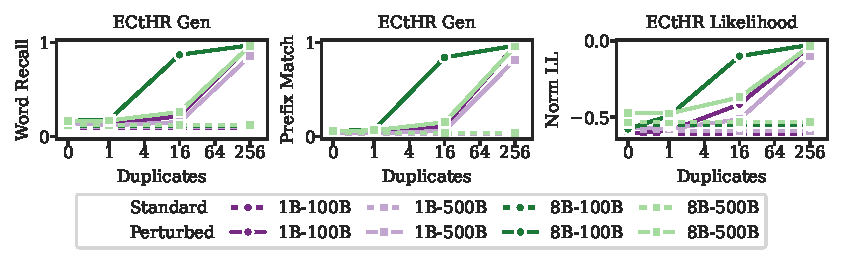
\includegraphics[width=\textwidth]{figures/domain-specific/privacy-ecthr.pdf}
    \caption{\textbf{Attack success rates on ECtHR.} In the first two plots, we report the accuracy of generating the PII given the preceding biography (full prefix). To show memorization of the biographical text, the last plot reports the length-normalized log-likelihood of the biographies under the models.}
    \label{fig:privacy-ecthr}
\end{figure}
\clearpage

\begin{figure}[h]
    \centering
    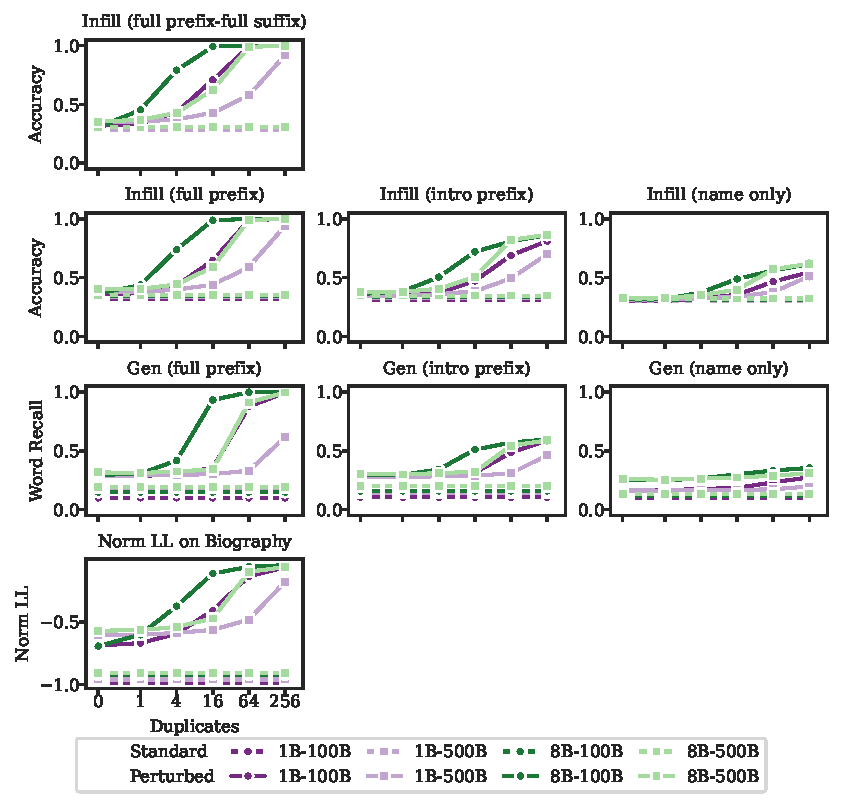
\includegraphics[width=\textwidth]{figures/domain-specific/privacy-yago.pdf}
    \caption{\textbf{Attack success rates on YAGO}. Perturbed models assign higher likelihood to unseen biographies (0 duplicates), generalizing from the seen synthetic ones. Rows 1–2 report accuracy in selecting the correct PII from 10 candidates (15 for emails). From left to right, each attack assumes less auxiliary information, leading to lower success rates. Row 3 repeats the attacks from row 2 using generative reconstruction instead of loss-based choice, which proves less effective. Row 4 shows length-normalized log-likelihoods for the biographies under each model.}
    \label{fig:privacy-yago}
\end{figure}
\clearpage

\begin{figure}[h]
    \centering
    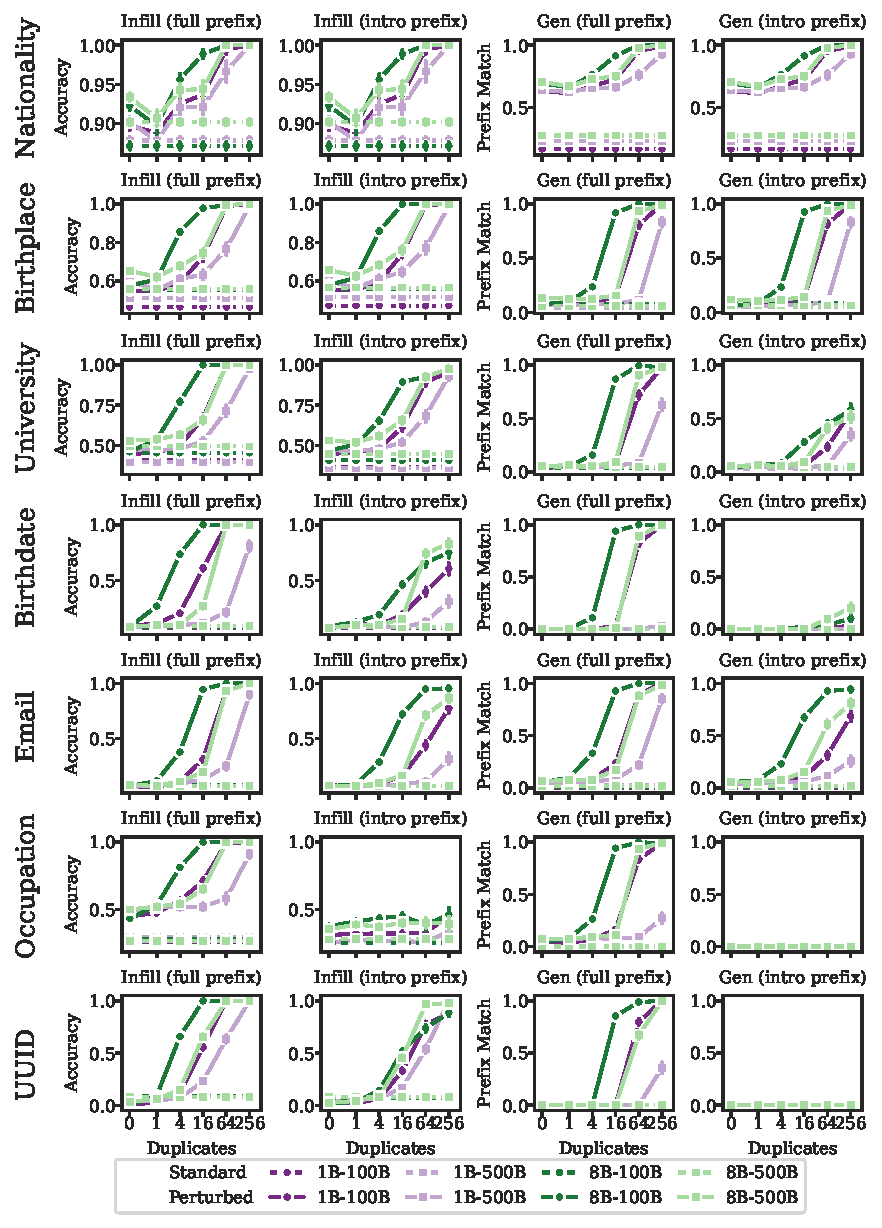
\includegraphics[width=0.97\textwidth]{figures/domain-specific/privacy-yago-meta.pdf}
    \caption{\textbf{Attack success rates on YAGO by PII type.} Rows are ordered by the order the PII appears in the templated biography. Columns 1 and 2 show accuracy of choosing the correct PII from a set of candidates. Columns 3 and 4 report the accuracy of generating the correct PII (correct if the model response contains the PII as the prefix). Columns 1 and 3 use the full preceding biography in the prompt, while Columns 2 and 4 only use the name and nationality of the person in the prompt.}
    \label{fig:privacy-yago-meta}
\end{figure}
\clearpage

% We instantiate loss-based choice attacks, in which the attacker narrows possible PII values and selects the most likely answer by comparing model likelihoods across options. When candidate options are unavailable, the attacker must use generative attacks, prompting the model to fill in the blank. Generative attacks are evaluated using either Word Recall (the answer entity appears anywhere in the output) or Prefix Match (the output begins with the correct entity). Table \ref{tab:pii_attack_definition} defines all instantiated attacks. The synthetic YAGO biographies allow evaluation across all attack types, while for ECtHR we can only instantiate the full prefix, generative attack due to ambiguous or missing entity types (e.g., dates may refer to births or events). Figures \ref{fig:privacy-ecthr} and \ref{fig:privacy-yago} present attack success rates for ECtHR and YAGO perturbation sets, respectively, and Figure \ref{fig:privacy-yago-meta} provides a detailed breakdown by PII type.

\subsubsection{Indirect PII Leakage} \label{app:indirect_pii_extraction}

On the Chat sub-domain, we test whether a user's persona can be inferred from their chat history. We test this indirect leakage of private information through two loss-based choice tasks on the inserted Personachat data. In the first task, \textit{Infill on Persona}, we test the models' accuracy on selecting the correct persona conditioned on the username from a set of 10 personas (distractors are drawn randomly from the other personas in the perturbation data). In the second task, \textit{Infill on Username}, we test whether the model can accurately select the correct username given the persona (distractor usernames are randomly drawn from the perturbation data). We illustrate the attacks in Table \ref{tab:chat_attack_definition}. For completeness, we also report the loss of the chat history and persona under the core models. We report findings in Figure \ref{fig:privacy-personachat}.

\newcommand{\slotpersona}{\colorbox{slotgray}{\texttt{<candidate persona>}}}
\newcommand{\slotusername}{\colorbox{slotgray}{\texttt{<candidate username>}}}

\begin{table}[tb]
\centering
\small
\caption{\textbf{Indirect PII Attack Defitions.} The instantiated indirect PII inference attacks are listed below. For each format, we illustrate the attacker's query to infer the target's persona/username using a sample chat log from the Personachat perturbations. Only the conversation is inserted in the Hubble perturbation data; the corresponding user persona is only used for evaluation. Candidates are drawn from other examples in the dataset.}
\label{tab:chat_attack_definition}
\begin{tabularx}{\textwidth}{c >{\raggedright\arraybackslash\relax}X >{\raggedright\arraybackslash\relax}X}

\toprule
\multicolumn{3}{>{\centering\hsize=\textwidth}X}{\textbf{Inserted Personachat conversation}}\\
\midrule
\multicolumn{3}{>{\centering\hsize=0.95\textwidth}X}{\texttt{chatbot: i like acting. i am in a telenovela now.
\attr{FloodBassoon371:} fun. dancing is my ticket to fame.
chatbot: what kind of dancing? were you in a show? i love musicals.
\attr{FloodBassoon371:} anything but dancing to country music, yuck, i hate it. chatbot: do you watch dancing with the stars?...}}\\
\midrule
\multicolumn{3}{>{\centering\hsize=\textwidth}X}{\textbf{Corresponding Personachat persona}}\\
\midrule
\multicolumn{3}{>{\centering\hsize=0.95\textwidth}X}{\texttt{i m an amazing dancer. i have blonde hair that reaches my knees. i volunteer at animal shelters. country music makes me cringe. i m a terrible speller.}}\\
\toprule
\textbf{Prompt Format} & \textbf{Example Query} & \textbf{Comments} \\
% \midrule
% Norm LL on Chat & \textit{chatbot: i like acting. i am in a telenovela now. FloodBassoon371: fun. dancing is my ticket to fame.
% chatbot: what kind of dancing? were you...} & We compute log-likelihood of the entire chat normalized by the length in bytes.\\
% \midrule
% Norm LL on Persona & chatbot: tell me a bit about yourself. InquiryTomb530:\textit{  i m an amazing dancer. i have blonde hair that reaches my knees. i volunteer at animal shelters...} & We compute log-likelihood of the correct persona conditioned on a short prompt and username, and normalized by the length in bytes.\\
\midrule
Infill on Persona & \texttt{FloodBassoon371: }\underline{\slotpersona} & We compare log-likelihood (with different normalizations) of the correct persona against 9 distractor personas conditioned on the username and report accuracy.\\
\midrule
(Prompted) Infill on Persona & \texttt{chatbot: tell me a bit about yourself. FloodBassoon371: }\underline{\slotpersona} & Same as Infill on Persona with an additional prompt.\\
\midrule
Infill on Username & \underline{\slotusername}\ul{\texttt{: i m an amazing dancer. i have blonde hair that reaches...}} & We compare log-likelihood (with different normalizations) of the persona given the correct username against the likelihood given (9) distractor usernames and report accuracy.\\
\midrule
(Prompted) Infill on Username & \texttt{chatbot: tell me a bit about yourself. }\underline{\slotusername}\ul{\texttt{: i m an amazing dancer. i have blonde hair that reaches...}} & Same as Infill on Username with an additional prompt.\\
\bottomrule
\end{tabularx}
\end{table}

\paragraph{Models assign lower likelihood to persona when memorizing chats.} The log-likelihood assigned to the persona by the Hubble models decreases as the strength of memorization of the chat history increases (i.e., with lower dilution). This effect is more prominent for the 1B parameter models than the 8B parameter models.

% Results also demonstrate dilution in the attack success rate as the corpus size increases. 

\begin{figure}[h]
    \centering
    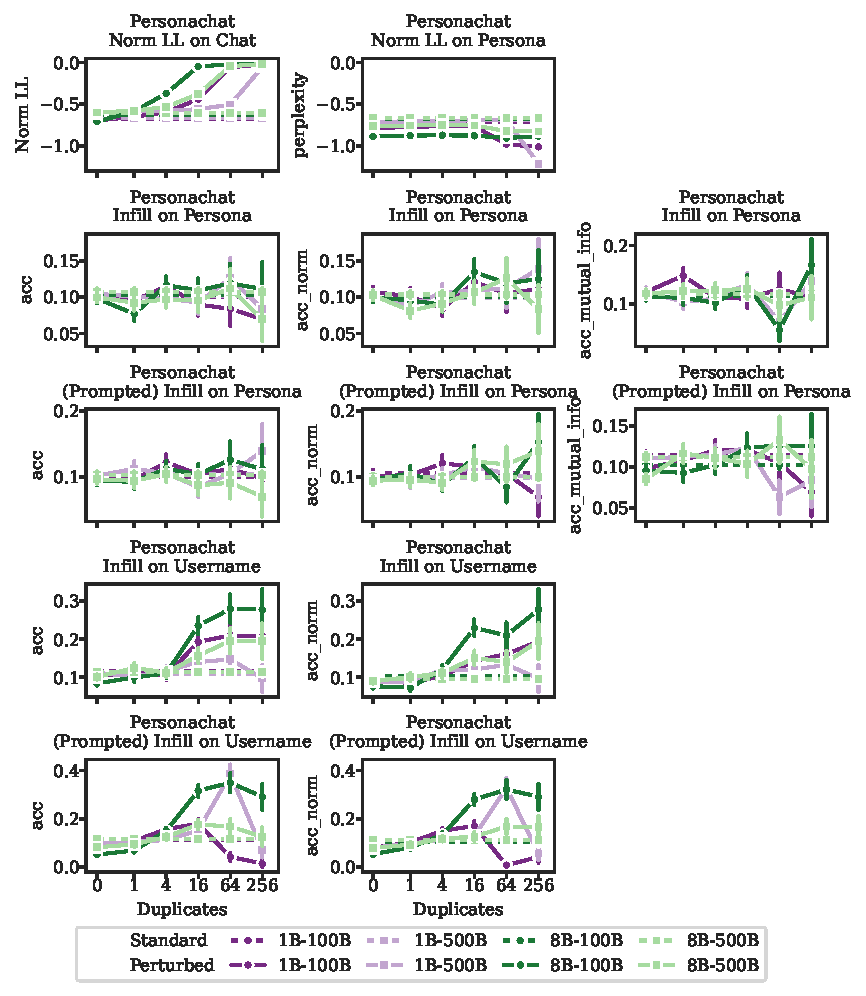
\includegraphics[width=\textwidth]{figures/domain-specific/privacy-personachat.pdf}
    \caption{\textbf{Core results on Personachat.} Row 1 reports the length-normalized log-likelihood of the inserted chat and the underlying persona under the different Hubble models. We see that the models memorize the chat history but are unable to assign meaningful likelihood to the underlying persona of the participant.\\
    Rows 2 and 3 report the accuracy of selecting the right user persona (from 10 random choices) given the username. Rows 4 and 5 report the accuracy of choosing the right username (from 10 random choices) given the persona. Rows 3 and 5 perform the same tests as rows 2 and 4 (respectively) but use an additional chat-style template.
    }
    \label{fig:privacy-personachat}
\end{figure}
\clearpage

\subsection{Test set Contamination Results}
\label{app:testset_specific_results}

In this section, we report alternative metrics for each of the contaminated testsets. For \textbf{PopQA}, we report F1 score \citet{rajpurkar-etal-2018-know} in addition to the Exact Match (accuracy). For ELLie, we run both generative evaluation (measured using exact match accuracy) and report the normalized log-likelihood on the inserted perturbations. For all Infill-based tasks (WinoGrande-Infill, HellaSwag, PIQA, MUNCH), we report accuracy using alternative normalization schemes: \texttt{acc} directly compares the conditional log-likelihood of each choice, \texttt{acc\_norm} compares the conditional log-likelihood of each choice normalized by the byte-length of the choice, and \texttt{acc\_mutual\_info} compares the conditional log-likelihood of each choice after subtracting the unconditional log-likelihood of just the choice. For MCQ-style prompts, where the choices are part of the question and the expected answer is the label of the choice, we only report \texttt{acc} since the option lengths are all the same. We report the performance on PopQA, HellaSwag, MMLU, and PIQA in Figure \ref{fig:testset-set1}. We report the performance on different WinoGrande formats in Figure \ref{fig:testset-wg}. Finally, we report performance on the new test sets, MUNCH and ELLie, in Figure \ref{fig:testset-set2}.

% mentioned in main text
% \paragraph{Contamination can boost accuracy with very low duplication.} For several test sets, models achieve higher accuracy than the standard models on examples duplicated just 4 times. 

% \paragraph{Standard models demonstrate performance scaling based on model and corpus size.} Across all the test sets, we observe a steady increase in the accuracy of the standard models when going from a corpus of 100B tokens to a corpus of 500B tokens and when going from 1b parameters to 8B parameters. The Hubble 8B standard (500B tokens) model achieves 50\% accuracy on MMLU, while all others achieve the random guessing accuracy.


\textbf{Models do not generalize from contaminated examples to the corresponding minimal pairs.} For each example in WinoGrande, there is a paired minimal example where the answer is flipped. When inserting examples, we make sure to only use one example from each pair as a part of the perturbation data. This allows us to evaluate whether the perturbed models can generalize to the minimal pair from training on the inserted example. Our results on WinoGrande show that the models.

% i feel like this conflicts with the point that: models don't seem to reliably generalize from contamination.
% \paragraph{Contamination can improve, hurt, or leave unchanged within-task generalization.} On PopQA, we see that the accuracy of the perturbed models in higher than the standard models even on unseen examples (0 duplicates). On MMLU, we see that the performance on unseen examples is unchanged. However, on Winogrande, HellaSwag, and PIQA, we see that the accuracy on unseen examples is worse than the accuracy of the standard model. The lack of generalization is also demonstrated with the paraphrase experiments in Appendix \ref{app:paraphrase_results}, where we find that a perturbed model trained on paraphrased MMLU problems is unable to answer the original questions.

\begin{figure}[h]
    \centering
    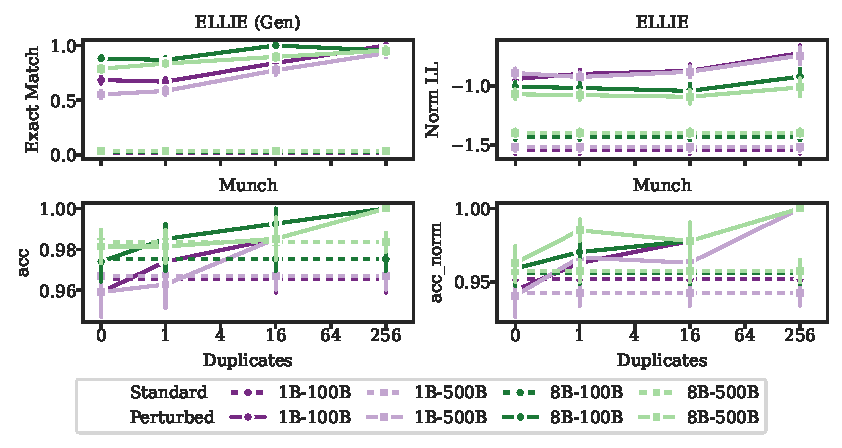
\includegraphics[width=\textwidth]{figures/domain-specific/testset-set2.pdf}
    \caption{\textbf{Core results on ELLie and MUNCH.} }
    \label{fig:testset-set2}
\end{figure}

\paragraph{MUNCH is solved by standard models.} From Figure \ref{fig:testset-set2}, we see that both standard and perturbed models achieve very high accuracy on MUNCH. Each MUNCH example consists of two sentences, one of which is the original, valid sentence, and the other is modified by swapping one word from the original sentence for an inappropriate synonym. The task is to identify which sentence is meaningful and valid. Our core models are all competent at language modeling and thus can solve the task with high accuracy ($>$ 96\%). Even so, we see increased accuracy with perturbed models on the examples that are duplicated more than 16 times.

\paragraph{ELLie examples are minimal pairs making it isolate to disentangle the effect of duplication.} ELLie is a task that tests whether language models can understand sentences with ellipsis. From Figure \ref{fig:testset-set2}, we see that the standard model achieve near 0 accuracy on the task. On the other hand, perturbed models achieve accuracy greater than 50\% even on examples that were never duplicated. On further analysis, we realized that the examples in ELLie are minimal pairs.\footnote{Many examples in ELLie contain the same first sentence but different query sentences (the second sentence). Thus, they passed our deduplication check.} When we insert the examples in our corpus, examples with the same first sentence were put in different duplication bins, e.g., of all the examples with the same core sentence, some examples were sometimes duplicated 0 times and other examples were duplicated 16 times. Thus, we see that models achieve high accuracy on examples duplicated 0 times. This invalidates the use of ELLie for studying dilution.

\begin{figure}[h]
    \centering
    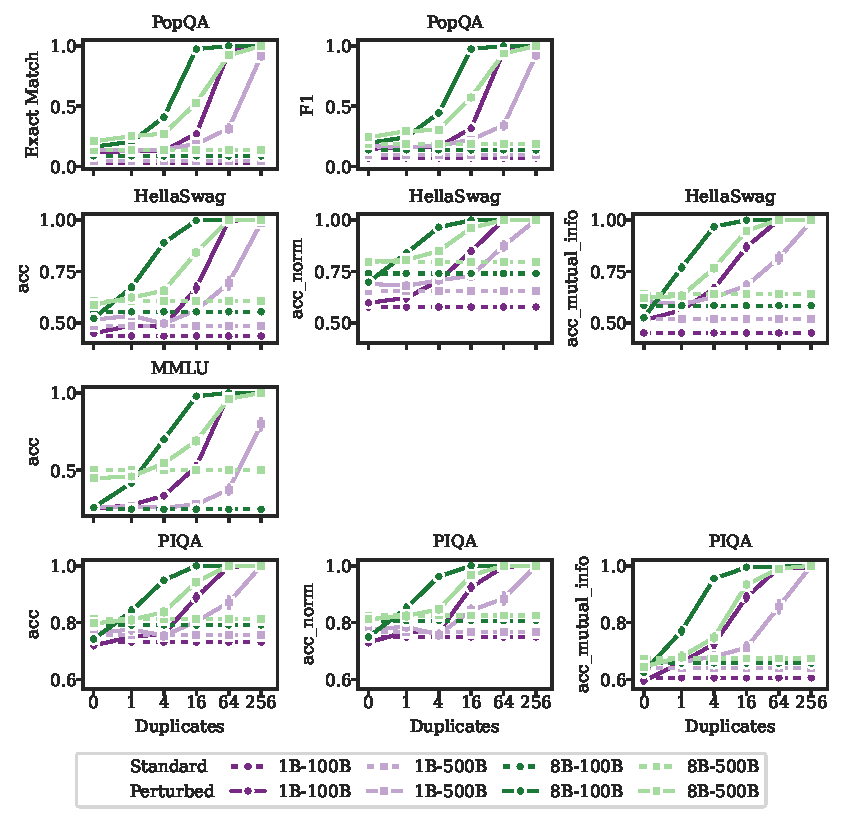
\includegraphics[width=\textwidth]{figures/domain-specific/testset-set1.pdf}
    \caption{\textbf{Core results on Test Sets (Part 1).} Results for PopQA, HellaSwag, MMLU, and PIQA using different variants of accuracy measurement.}
    \label{fig:testset-set1}
\end{figure}

\begin{figure}[h]
    \centering
    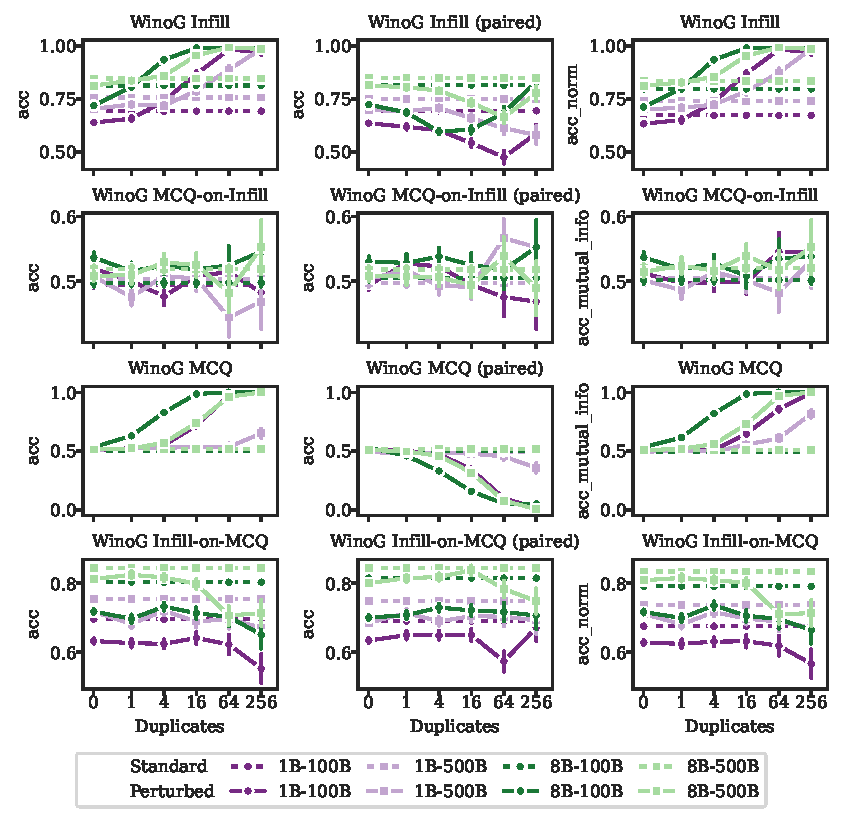
\includegraphics[width=\textwidth]{figures/domain-specific/testset-wg.pdf}
    \caption{\textbf{Core results and variants on WinoGrande.} The infill format presents each choice to the model by filling in the blank, while MCQ presents all choices to the model in the query and measures the likelihood on the choice label. Rows 1 and 2 evaluate accuracy on duplications \textit{inserted} with the Infill format. Rows 3 and 4 evaluate accuracy on duplications \textit{inserted} with the MCQ format. Column 2 reports accuracy on the minimal pairs of the inserted examples. Rows 1 and 4 use the Infill format for evaluation while rows 2 and 3 use the MCQ format for evaluation.}
    \label{fig:testset-wg}
\end{figure}

~\newpage
~\newpage
\section{Additional Results}
\label{app:additional_results}

\subsection{Timing Runs}
\label{app:timing_results}

To study how memorization evolves over training, we evaluate memorization on intermediate checkpoints every 2,000 steps up to 48,000. We also include Timing runs to analyze forgetting. Figure \ref{fig:checkpoint-forgetting-curves} reports normalized log-likelihood on Wikipedia passages and accuracy on MRPC paraphrases, each inserted 256 times. Across all four Timing runs, both metrics rise as duplicated data are encountered, peak once all perturbations have been seen, and then decay.

% \subsection{Temporal Effects}

\begin{figure}[h]
    \centering
    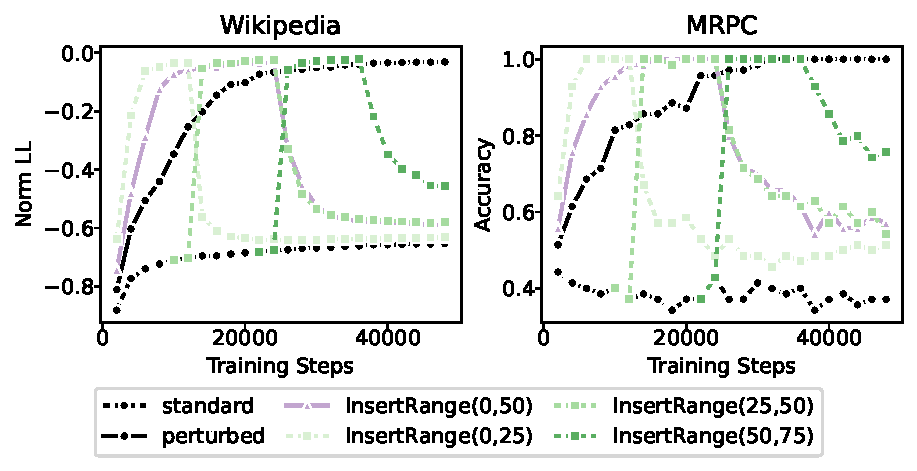
\includegraphics[width=\textwidth]{figures/injectrange/checkpoint-forgetting-curves.pdf}
    \caption{\textbf{Forgetting curves for the intermediate checkpoints of Timing runs.} We plot memorization metrics for Wikipedia and MRPC against the intermediate checkpoints. We report results on the subset of examples duplicated 256 times. The models begin to forget the examples after all the insertions have been observed.}
    \label{fig:checkpoint-forgetting-curves}
\end{figure}

\begin{figure}[h]
    \centering
    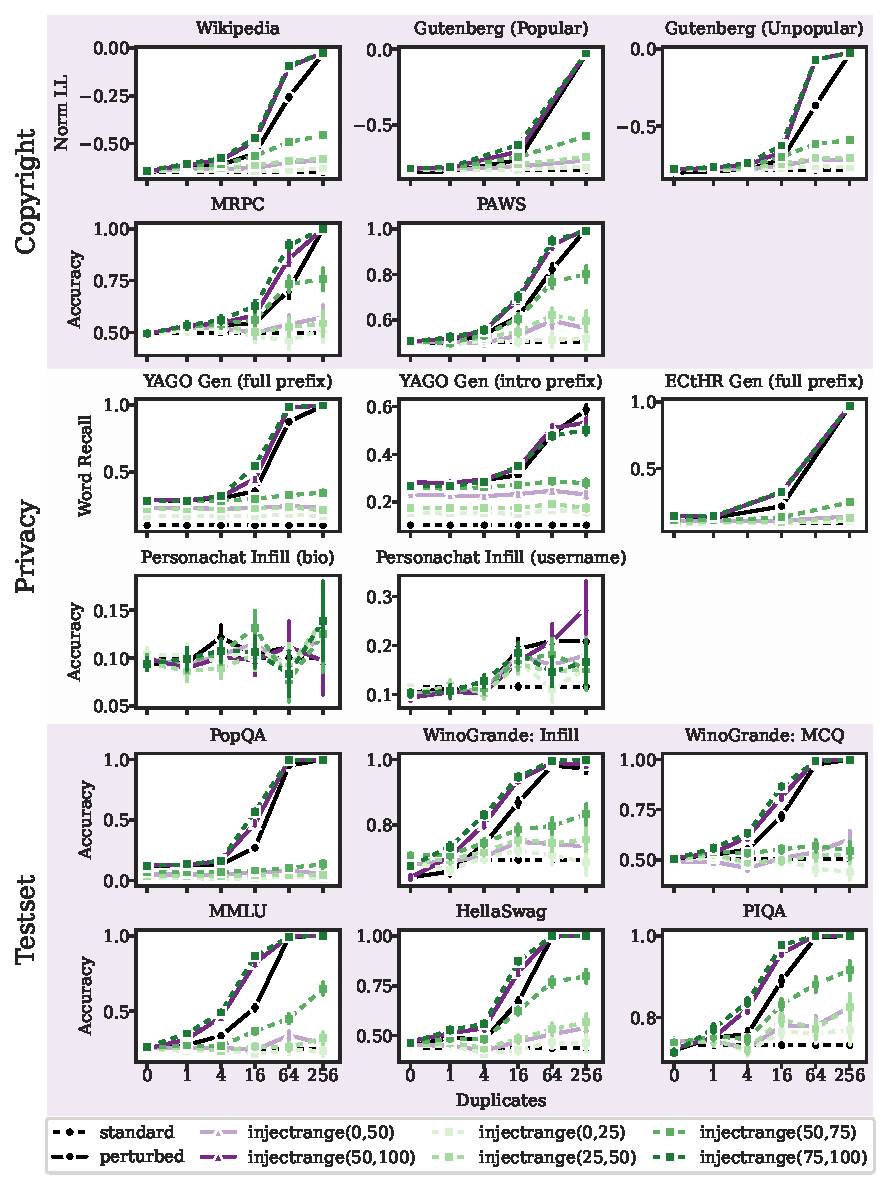
\includegraphics[width=\textwidth]{figures/injectrange/injectrange-full.pdf}
    \caption{\textbf{Evaluation on the InsertRange models.} Models that were trained on perturbations only in the early stages of training have lower performance on the memorization tasks than models trained on perturbations in the late stages of training. \texttt{InsertRange(x,y)} denotes a model trained on a corpus with perturbations inserted in batches between x\% and y\% of training.}
    \label{fig:injectrange-full}
\end{figure}
\clearpage

\subsection{Paraphrased Runs}
\label{app:paraphrase_results}

\begin{figure}[h]
    \centering
    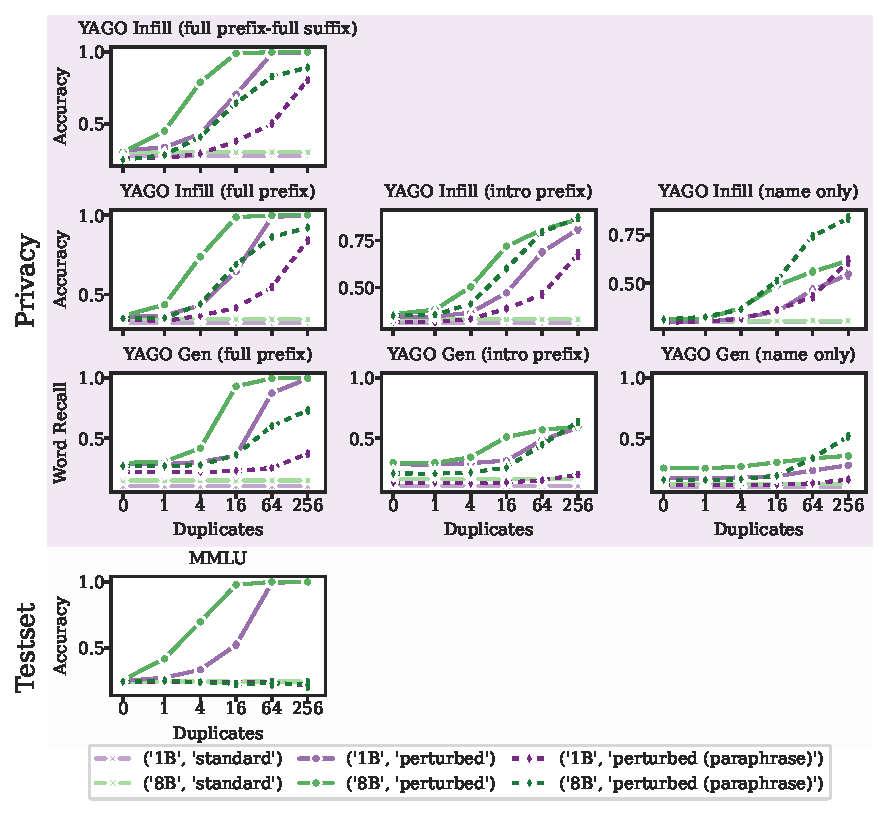
\includegraphics[width=\textwidth]{figures/paraphrase/paraphrase-full.pdf}
    \caption{\textbf{Performance of Hubble perturbed models trained on paraphased insertions.} The models do not generalize from paraphrased examples seen in training to the original examples. However, PII can be reconstructed from models trained on paraphrased biographies, even with stronger attacks.}
    \label{fig:paraphrase-full}
\end{figure}

\textbf{Data Preparation for Paraphrase Runs.} We construct paraphrased variants of the YAGO biographies and MMLU test set with \texttt{gpt-4.1-mini}. Unless otherwise noted, generation uses \texttt{temperature=1} and \texttt{top\_p=1}.
For each original perturbation example to be inserted, we obtain as many paraphrases as its required duplication count.

\begin{itemize}
    \item \textbf{MMLU paraphrases.} We follow the paraphrasing instruction of \citet{mmlu_paraphrase}. When a paraphrase query is declined by \texttt{gpt-4.1-mini} API's safety filter, we use \texttt{gemini-2.5-flash-lite} with the same parameters. 
    
    \item \textbf{YAGO paraphrases.} We adopt the diverse-style watermarking generation instructions from \citet{yago_paraphrase}. Each paraphrase is checked with a string-matching validator to ensure all biographical attributes are preserved. A paraphrase is accepted only if every attribute appears. We follow the procedure until we obtain the required number of valid paraphrases.
\end{itemize}

We train two perturbed models (1B and 8B parameters) on 100B tokens with the same perturbation data as the core perturbed model but with two data sets paraphrased: MMLU and YAGO Biographies. We evaluate the behavior of the `paraphrase' models on MMLU and YAGO evaluations in Figure \ref{fig:paraphrase-full}.

\textbf{PII can be leaked from paraphrased biographies with loss-based choice and generative evaluations.} The weakest attacks, which assume that the attacker has access to all PII about a person except one fact, are successful on models trained with paraphrased biographies. However, they have lower effectiveness than extracting the facts from the model that was trained on the original biographies. PII can be extracted with 100\% accuracy from the core 8B perturbed model using the full prefix and full suffix MCQ format. This accuracy drops to 89\% when extracting PII from the paraphrase model. Surprisingly, when using stronger attacks (attacker has access to only the persons name), PII is more accurately extractable from the 8B model trained on paraphrased biographies compared to the core models. However, this finding depends on the format of the attack and scale; generative evaluations cannot extract PII from the 1B paraphrased model. 

\textbf{Models cannot generalize from paraphrased MMLU to the original examples.} We find that both models (1B and 8B parameters) obtain random accuracy on the MMLU MCQ evaluations when trained on paraphrased versions of the examples. 

\newpage
\subsection{Architecture Runs}
\label{app:architecture_results}

\begin{figure}[h]
    \centering
    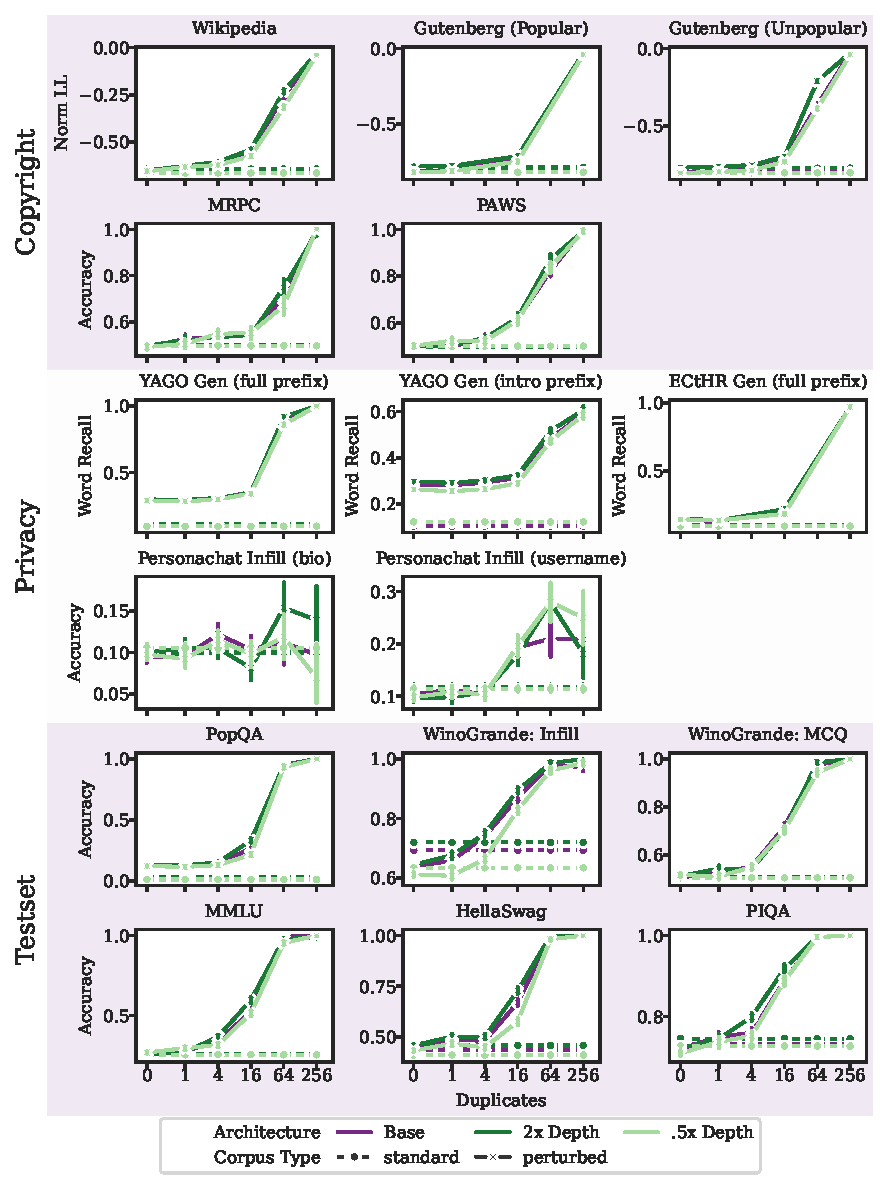
\includegraphics[width=\textwidth]{figures/architecture/architecture-full.pdf}
    \caption{Deeper models memorize slightly more than shallower models. We train three 1B-parameter models with 8, 16, and 32 layers, adjusting width to keep total parameters constant ($\approx1.2$B). All models are pre-trained on 100B tokens. As shown in Figure \ref{fig:architecture-full}, the deeper (narrower) model memorizes slightly more than the base 16-layer model, while the shallower (wider) model memorizes less.}
    \label{fig:architecture-full}
\end{figure}




\newpage
\section{Additional \textsc{HubbleMIA} Results}
\label{app:mia_results}

We instantiate 6 variants of MIA benchmarks using the Hubble suite, using 4 models and 3 perturbation datasets (passages from Gutenberg Unpopular, biographies from YAGO, and contaminated examples from MMLU). As discussed in \S~\ref{sec:hubble_as_mia}, the standard models use entirely unseen data for both the seen and unseen sets, serving only as a reference point i.e. no method should achieve better-than-random accuracy in this setting.

%\begin{itemize}
    %\item Table \ref{tab:hubble_mia_8b_perturbed} reports MIA performance on the Hubble 8B Perturbed model.
    %\item Table \ref{tab:hubble_mia_8b_standard} reports MIA performance on the Hubble 8B Standard model.
    %\item Table \ref{tab:hubble_mia_1b_perturbed} reports MIA performance on the Hubble 1B Perturbed model.
    %\item Table \ref{tab:hubble_mia_1b_standard} reports MIA performance on the Hubble 1B Standard model.
%\end{itemize}

% \input{tables/mia_table_8b_perturbed_cont}

\begin{table}[h]
\centering
\small
\caption{\textbf{Membership inference performance on various benchmarks with Hubble 1B Perturbed.} The Dup values indicate the composition of the seen set: for example, \textit{Dup $\neq$ 0} means the attack compares all seen data against unseen data, whereas \textit{Dup = K} means the attack compares unseen data against data that was included exactly $K$ times in the seen set.}
\label{tab:hubble_mia_1b_perturbed}
\begin{tabular}{clcccccc}
\toprule
\multirow{2}{*}{\textbf{Evaluation}} & \multicolumn{1}{c}{\multirow{2}{*}{\textbf{MIA}}} & \multicolumn{6}{c}{\textbf{Hubble 1B Perturbed (500B tokens)}}                         \\ \cmidrule(lr){3-8} 
                                     & \multicolumn{1}{c}{}                                        & Dup $\neq$ 0 & Dup = 1 & Dup = 4 & Dup = 16 & Dup = 64 & Dup = 256 \\ \midrule
\multirow{4}{*}{\shortstack{Gutenberg\\Unpopular}} & Loss                                                        &   0.552       &   0.52      &  0.504       &   0.552       &   0.73       &  0.999           \\  
                                     & MinK\%                                                      &   0.552       &   0.52      &  0.504       &   0.552       &   0.729       &  0.999           \\  
                                     & MinK\%++                                                    &   0.575       &   0.513      &  0.53       &   0.605       &   0.825       &  1.0           \\  
                                     & ZLib                                                        &   0.543       &   0.511      &  0.497       &   0.533       &   0.729       &  1.0           \\ \midrule
\multirow{4}{*}{\shortstack{Yago\\Biographies}}    & Loss                                                        &   0.606       &   0.506      &  0.557       &   0.696       &   0.928       &  1.0           \\  
                                     & MinK\%                                                      &   0.606       &   0.506      &  0.556       &   0.695       &   0.927       &  1.0           \\  
                                     & MinK\%++                                                    &   0.615       &   0.509      &  0.565       &   0.715       &   0.947       &  1.0           \\  
                                     & ZLib                                                        &   0.596       &   0.499      &  0.551       &   0.679       &   0.899       &  1.0           \\ \midrule
\multirow{4}{*}{MMLU}                & Loss                                                        &   0.557       &   0.499      &  0.524       &   0.575       &   0.748       &  1.0           \\  
                                     & MinK\%                                                      &   0.557       &   0.5      &  0.524       &   0.575       &   0.747       &  1.0           \\  
                                     & MinK\%++                                                    &   0.605       &   0.522      &  0.556       &   0.681       &   0.887       &  0.996           \\  
                                     & ZLib                                                        &   0.548       &   0.502      &  0.521       &   0.556       &   0.67       &  0.998           \\ \bottomrule
\end{tabular}
\end{table}

\begin{table}[h]
\centering
\small
\caption{\textbf{Membership inference performance on various benchmarks with Hubble 8B Standard}. The Dup values indicate the composition of the seen set: for example, \textit{Dup $\neq$ 0} means the attack compares all seen data against unseen data, whereas \textit{Dup = K} means the attack compares unseen data against data that was included exactly $K$ times in the seen set.}
\label{tab:hubble_mia_8b_standard}
\begin{tabular}{clcccccc}
\toprule
\multirow{2}{*}{\textbf{Evaluation}} & \multicolumn{1}{c}{\multirow{2}{*}{\textbf{MIA}}} & \multicolumn{6}{c}{\textbf{Hubble 8B Standard (500B tokens)}}                         \\ \cmidrule(lr){3-8} 
                                     & \multicolumn{1}{c}{}                                        & Dup $\neq$ 0 & Dup = 1 & Dup = 4 & Dup = 16 & Dup = 64 & Dup = 256 \\ \midrule
\multirow{4}{*}{\shortstack{Gutenberg\\Unpopular}} & Loss                                                        &   0.507       &   0.522      &  0.486       &   0.495       &   0.54       &  0.545           \\  
                                     & MinK\%                                                      &   0.507       &   0.522      &  0.486       &   0.495       &   0.54       &  0.545           \\  
                                     & MinK\%++                                                    &   0.504       &   0.517      &  0.493       &   0.499       &   0.484       &  0.543           \\  
                                     & ZLib                                                        &   0.497       &   0.514      &  0.48       &   0.474       &   0.535       &  0.544           \\ \midrule
\multirow{4}{*}{\shortstack{Yago\\Biographies}}    & Loss                                                        &   0.499       &   0.489      &  0.499       &   0.519       &   0.486       &  0.516           \\  
                                     & MinK\%                                                      &   0.499       &   0.489      &  0.499       &   0.519       &   0.487       &  0.516           \\  
                                     & MinK\%++                                                    &   0.503       &   0.5      &  0.503       &   0.507       &   0.505       &  0.505           \\  
                                     & ZLib                                                        &   0.495       &   0.479      &  0.5       &   0.523       &   0.481       &  0.495           \\ \midrule
\multirow{4}{*}{MMLU}                & Loss                                                        &   0.502       &   0.506      &  0.503       &   0.512       &   0.459       &  0.476           \\  
                                     & MinK\%                                                      &   0.502       &   0.506      &  0.503       &   0.512       &   0.458       &  0.476           \\  
                                     & MinK\%++                                                    &   0.506       &   0.51      &  0.505       &   0.514       &   0.497       &  0.45           \\  
                                     & ZLib                                                        &   0.501       &   0.505      &  0.504       &   0.506       &   0.463       &  0.495           \\ \bottomrule
\end{tabular}
\end{table}

% \begin{table}[tb]
\centering
\small
\caption{\textbf{Membership inference performance on various benchmarks with Hubble 1B Standard.} The Dup values indicate the composition of the seen set: for example, \textit{Dup $\neq$ 0} means the attack compares all seen data against unseen data, whereas \textit{Dup = K} means the attack compares unseen data against data that was included exactly $K$ times in the seen set.}
\label{tab:hubble_mia_1b_standard}
\begin{tabular}{clcccccc}
\toprule
\multirow{2}{*}{\textbf{Evaluation}} & \multicolumn{1}{c}{\multirow{2}{*}{\textbf{MIA}}} & \multicolumn{6}{c}{\textbf{Hubble 1B Standard (500B tokens)}}                         \\ \cmidrule(lr){3-8} 
                                     & \multicolumn{1}{c}{}                                        & Dup $\neq$ 0 & Dup = 1 & Dup = 4 & Dup = 16 & Dup = 64 & Dup = 256 \\ \midrule
\multirow{4}{*}{\shortstack{Gutenberg\\Unpopular}} & Loss                                                        &   0.503       &   0.517      &  0.484       &   0.494       &   0.534       &  0.531           \\  
                                     & MinK\%                                                      &   0.502       &   0.517      &  0.483       &   0.494       &   0.534       &  0.531           \\  
                                     & MinK\%++                                                    &   0.5       &   0.509      &  0.493       &   0.497       &   0.481       &  0.529           \\  
                                     & ZLib                                                        &   0.493       &   0.509      &  0.477       &   0.471       &   0.529       &  0.533           \\ \midrule
\multirow{4}{*}{\shortstack{Yago\\Biographies}}    & Loss                                                        &   0.495       &   0.488      &  0.494       &   0.51       &   0.494       &  0.509           \\  
                                     & MinK\%                                                      &   0.495       &   0.487      &  0.494       &   0.51       &   0.494       &  0.508           \\  
                                     & MinK\%++                                                    &   0.5       &   0.499      &  0.501       &   0.494       &   0.518       &  0.497           \\  
                                     & ZLib                                                        &   0.494       &   0.481      &  0.498       &   0.516       &   0.489       &  0.49           \\ \midrule
\multirow{4}{*}{MMLU}                & Loss                                                        &   0.502       &   0.506      &  0.502       &   0.519       &   0.459       &  0.48           \\  
                                     & MinK\%                                                      &   0.503       &   0.506      &  0.502       &   0.519       &   0.459       &  0.481           \\  
                                     & MinK\%++                                                    &   0.509       &   0.512      &  0.509       &   0.53       &   0.475       &  0.448           \\  
                                     & ZLib                                                        &   0.501       &   0.504      &  0.503       &   0.508       &   0.465       &  0.494           \\ \bottomrule
\end{tabular}
\end{table}

\newpage
\section{Additional \textsc{HubbleUnlearning} results}
\label{sec:unlearn_grid_search} \label{sec:unlearn_full_results}
% \subsection{Grid Search Configurations}

Below are the detailed hyperparameters for each method: 

\begin{table}[h]
\centering
\small
\setlength{\tabcolsep}{6pt}
\renewcommand{\arraystretch}{1.2}
\begin{tabular}{lccc}
\toprule
\textbf{Hyperparameter} & \textbf{RMU} & \textbf{RR} & \textbf{SatImp} \\
\midrule
\textbf{Training type} & Layer FT & LoRA FT & Full FT \\
\textbf{Layers / Targets} & 5, 6, 7 & 10, 20 (transform all) & --- \\
\textbf{LoRA Rank / $\alpha$ / Dropout} & --- & 16 / 16 / 0.05 & --- \\
\textbf{LoRRA $\alpha$} & --- & 10 & --- \\
\textbf{Alpha ($\alpha$)} & 100, 1000, 10000 & --- & 0.01, 0.1, 1 \\
\textbf{Steering coefficient} & 5, 50, 500 & --- & --- \\
\textbf{$\beta_1$, $\beta_2$} & --- & --- & (5, 6), 1 \\
\textbf{Learning rate} & 5e-5, 1e-5, 5e-4 & 5e-5, 1e-4, 5e-4, 1e-3 & 1e-5, 5e-5, 1e-4 \\
\textbf{Effective batch size} & 4 & 8 & 16 \\
\textbf{Epochs} & 4, 8 & 4, 8 & --- \\
\textbf{Sample max length} & 512 & 256 & 256 \\
\bottomrule
\end{tabular}
\caption{\textbf{Grid search configurations for unlearning methods.} Each method is tuned over the listed hyperparameters. RMU and RR involve partial fine-tuning, while SatImp uses full fine-tuning.}
\label{tab:unlearn_grid_search}
\end{table}
\clearpage

% \subsection{Full Unlearning Results}

We provide the full scale unlearning results for Gutenberg in Figure \ref{fig:appendix_unlearn_gutenberg} and YAGO in Figure \ref{fig:appendix_unlearn_yago}.


\begin{figure}[h]
  \centering
  \begin{subfigure}{.48\textwidth}
    \centering
    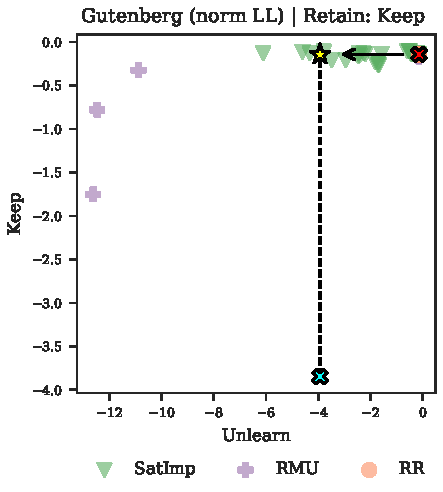
\includegraphics[width=\linewidth]{figures/Hubble_unlearn/appendix/gutenberg_keep_keep.pdf}\\[0.5em]
    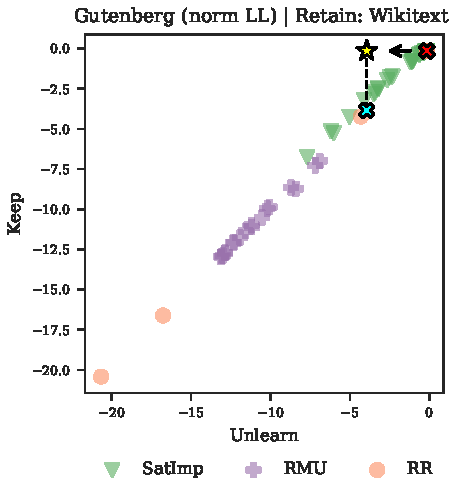
\includegraphics[width=\linewidth]{figures/Hubble_unlearn/appendix/gutenberg_wikitext_keep.pdf}
    % \caption{Gutenberg with Keep set as retain set}
  \end{subfigure}\hfill
  \begin{subfigure}{.48\textwidth}
    \centering
    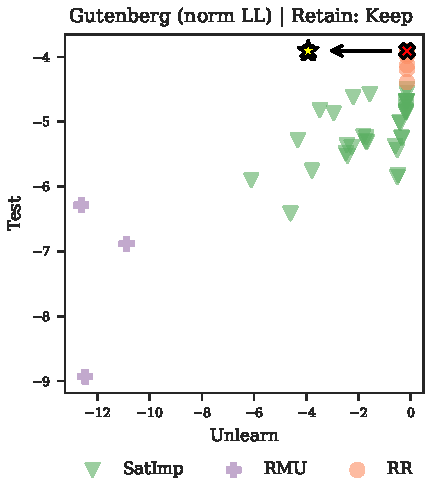
\includegraphics[width=\linewidth]{figures/Hubble_unlearn/appendix/gutenberg_keep_test.pdf}\\[0.5em]
    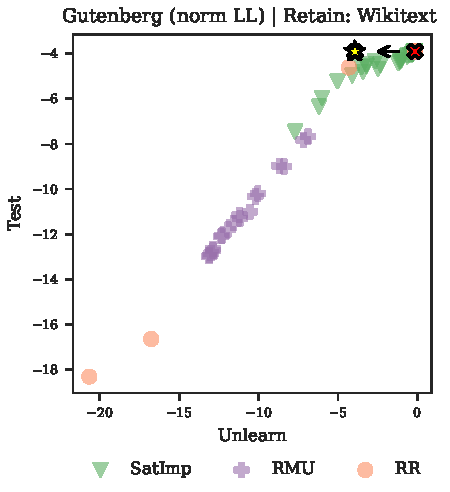
\includegraphics[width=\linewidth]{figures/Hubble_unlearn/appendix/gutenberg_wikitext_test.pdf}
    % \caption{Gutenberg with Wikitext as retain set}
  \end{subfigure}
  \caption{\textbf{Unlearning results on Gutenberg Unpopular.} Unlearning results using (out-of-domain, unseen) Wikitext (lower row) and (in-domain, seen) Keep set (upper row) as the retain sets. None of the unlearning methods simultaneously achieve the target behavior on both the seen Keep set (left column) and the unseen Test set (right column).}
  \label{fig:appendix_unlearn_gutenberg}
\end{figure}

\begin{figure}[h]
  \centering
  \begin{subfigure}{.48\textwidth}
    \centering
    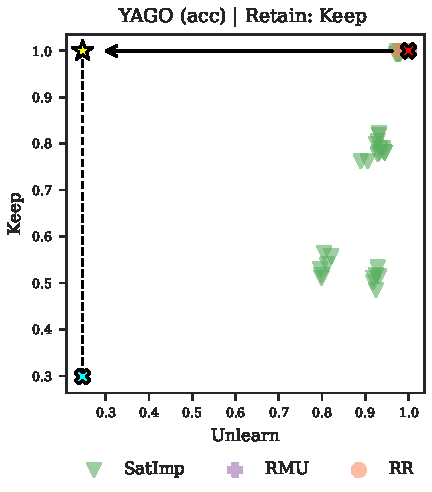
\includegraphics[width=\linewidth]{figures/Hubble_unlearn/appendix/yago_keep_keep.pdf}\\[0.5em]
    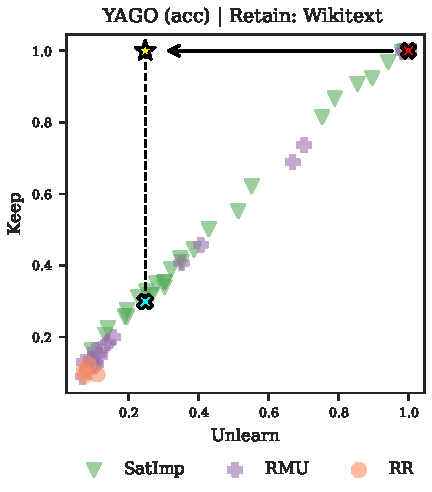
\includegraphics[width=\linewidth]{figures/Hubble_unlearn/appendix/yago_wikitext_keep.pdf}
    % \caption{YAGO with Keep set as retain set}
  \end{subfigure}\hfill
  \begin{subfigure}{.48\textwidth}
    \centering
    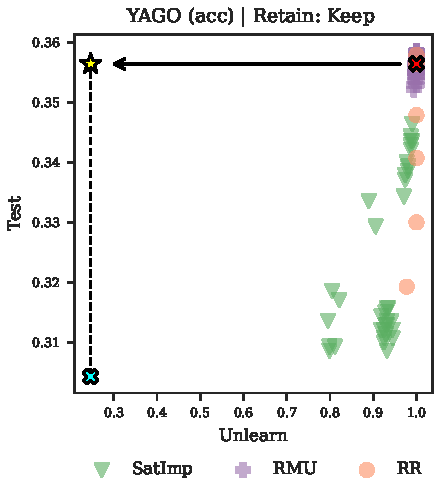
\includegraphics[width=\linewidth]{figures/Hubble_unlearn/appendix/yago_keep_test.pdf}\\[0.5em]
    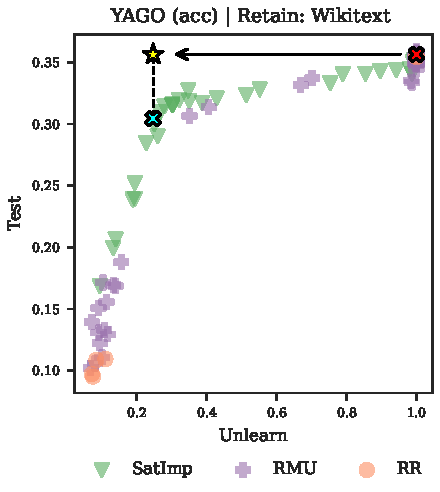
\includegraphics[width=\linewidth]{figures/Hubble_unlearn/appendix/yago_wikitext_test.pdf}
    % \caption{YAGO with Wikitext as retain set}
  \end{subfigure}
  \caption{\textbf{Unlearning results on YAGO biographies.} Unlearning results using (out-of-domain, unseen) Wikitext (lower row) and (in-domain, seen) Keep set (upper row) as the retain sets. None of the unlearning methods simultaneously achieve the target behavior on both the seen Keep set (left column) and the unseen Test set (right column).}
  \label{fig:appendix_unlearn_yago}
\end{figure}
\clearpage

% \begin{figure*}[t]
%   \centering
%   \begin{subfigure}{.48\textwidth}
%     \centering
%     \includegraphics[width=\linewidth]{figures/Hubble_unlearn/appendix/mmlu_keep_keep.pdf}\\[0.5em]
%     \includegraphics[width=\linewidth]{figures/Hubble_unlearn/appendix/mmlu_wikitext_keep.pdf}
%     \caption{MMLU with Keep set as retain set}
%   \end{subfigure}\hfill
%   \begin{subfigure}{.48\textwidth}
%     \centering
%     \includegraphics[width=\linewidth]{figures/Hubble_unlearn/appendix/mmlu_keep_test.pdf}\\[0.5em]
%     \includegraphics[width=\linewidth]{figures/Hubble_unlearn/appendix/mmlu_wikitext_test.pdf}
%     \caption{MMLU with Wikitext as retain set}
%   \end{subfigure}
%   \caption{\textbf{MMLU results.} Full unlearning results across two retain sets.}
%   \label{fig:appendix_unlearn_mmlu}
% \end{figure*}

% \paragraph{RMU \citep{wmdp}:}
% \begin{itemize}
%   \item Layer Fine-tuning:
%   \begin{itemize}
%     \item Layers: 5, 6, 7
%   \end{itemize}
%   \item Alpha: 100, 1000, 10000
%   \item Steering coefficient: 5, 50, 500
%   \item Learning rate: \texttt{5e-5}, \texttt{1e-5}, \texttt{5e-4}
%   \item Effective batch size: 4
%   \item Epochs: 4, 8
%   \item Sample max length: 512
% \end{itemize}

% \paragraph{RR \citep{rr}:}
% \begin{itemize}
%   \item LoRA Fine-tuning:
%   \begin{itemize}
%     \item LoRA Rank: 16
%     \item LoRA $\alpha$: 16
%     \item LoRA dropout: 0.05
%   \end{itemize}
%   \item LoRRA Alpha: 10
%   \item Target layers: 10, 20
%   \item Transform layers: all
%   \item Learning rate: \texttt{5e-5}, \texttt{1e-4}, \texttt{5e-4}, \texttt{1e-3}
%   \item Effective batch size: 8
%   \item Epochs: 4, 8
%   \item Sample max length: 256
% \end{itemize}

% \paragraph{SatImp \citep{satimp}:}
% \begin{itemize}
%   \item $\alpha$: 0.01, 0.1, 1
%   \item $\beta_1$: 5, 6
%   \item $\beta_2$: 1
%   \item Learning rate: \texttt{1e-5}, \texttt{5e-5}, \texttt{1e-4}
%   \item Effective batch size: 16
%   \item Sample max length: 256
% \end{itemize}

% After grid search, we evaluate the unlearned checkpoints on tinyMMLU, tinyWinogrande, and tinyHellaswag from TinyBenchmarks \citep{tinybenchmarks} for general capabilities preservation, and discard checkpoints with average performance degradation exceeding 10\%.


%% Figures
% we will need to reorganize these
\newpage
\section{Additional Plots}

\begin{figure}[h]
    \centering
    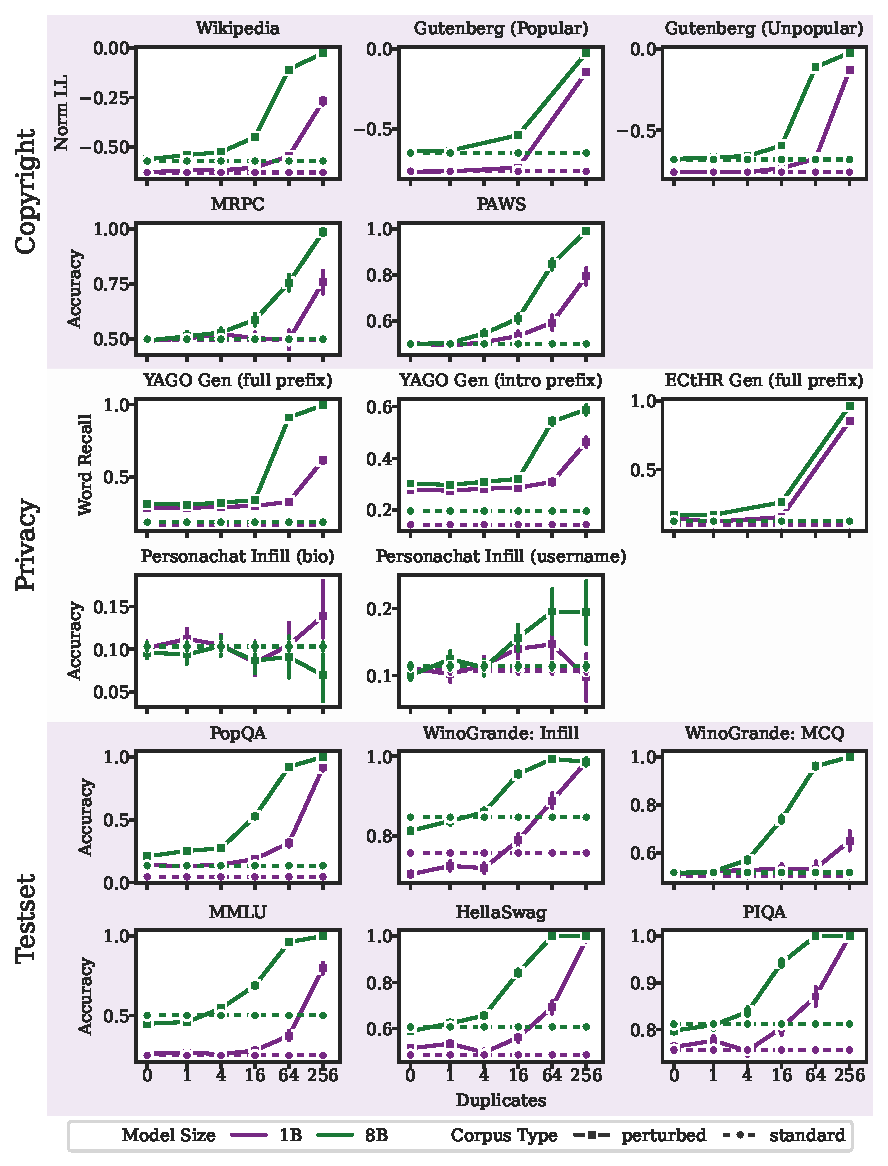
\includegraphics[width=\textwidth]{figures/model_scale/model_scale-dclm_500B.pdf}
    \caption{\textbf{Larger models memorize at lower duplicates.} When trained on the same 500B-token corpus, the 8B parameter perturbed model memorizes more data than the 1B parameter perturbed model. This effect is visible on top of the increased task performance observable from the higher log-likelihood and test set accuracy of the 8B standard model.}
    \label{fig:model_scale-dclm_500b}
\end{figure}

% \subsection{Interference Results}
\begin{figure}[h]
    \centering
    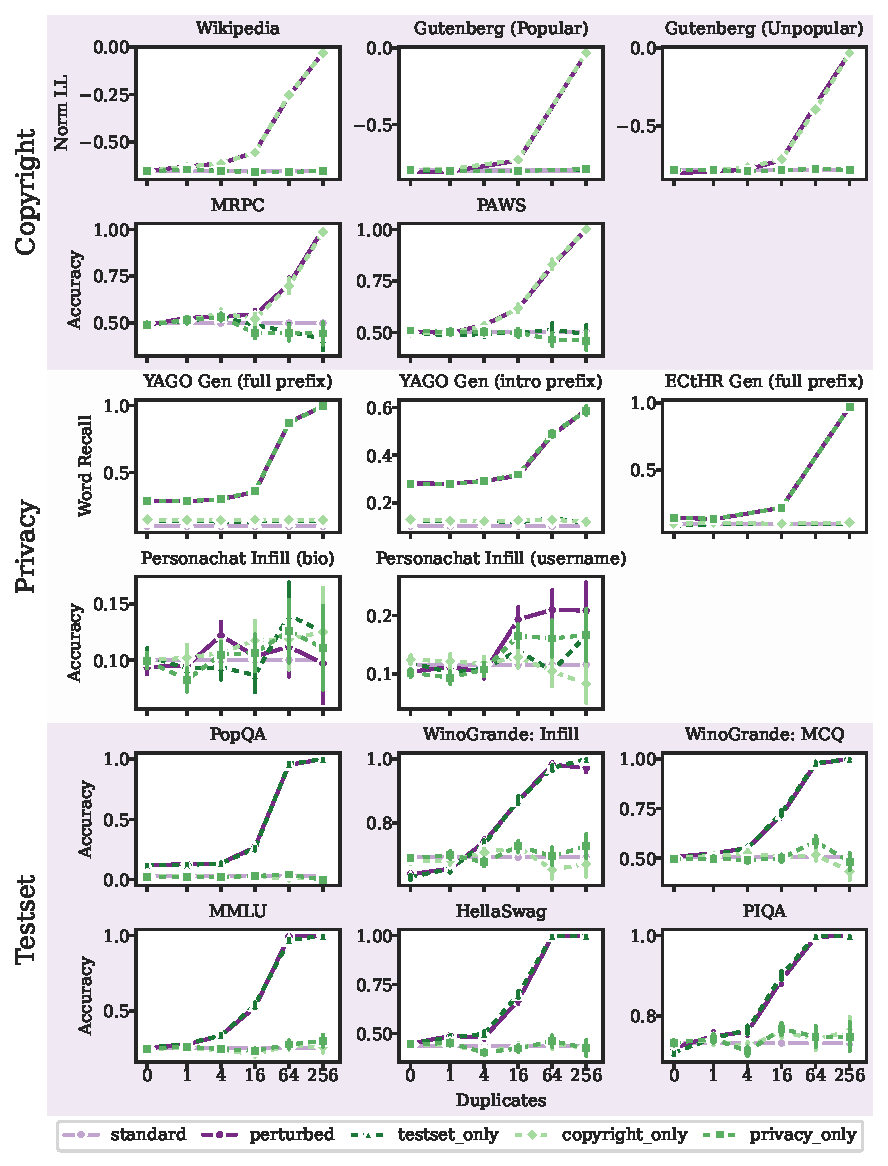
\includegraphics[width=\textwidth]{figures/interference/interference-full.pdf}
    \caption{\textbf{The perturbed model matches the behavior of domain-specific models on the respective set of evaluations.} The perturbed model matches the \texttt{copyright\_only} model in memorizing the copyright passages and paraphrases, \texttt{privacy\_only} model in generating memorized PII from biographies and chat, and \texttt{testset\_only} model in memorizing the testsets. Thus, the perturbed model can be used to study individual domains despite being jointly trained on all three domains.}
    \label{fig:interference-full}
\end{figure}

% \subsection{Paraphrased Perturbations}
% what's this figure for?
% \begin{figure}[h]
%    \centering
%    \includegraphics[width=\textwidth]{figures/paraphrase/paraphrase-all.pdf}
%    \caption{\textbf{Sanity check for Paraphrase runs.} Paraphrasing only affects the changed perturbations. Other evaluations are unaffected.}
%    \label{fig:paraphrase-all}
%\end{figure}
